\chapter{The Phase-2 Upgrade of the CMS Detector}
\label{chap:Upgrade}

Planned to start in 2029, the \ac{HL-LHC}~\cite{Apollinari:2017lan} will reach a peak instantaneous luminosity of up to $7.5\times10^{34}$cm$^{-2}$s$^{-1}$, as illustrated in Figure~\ref{fig:Lumi}. The increased luminosity will open up opportunities for ambitious physics programs including precision \ac{SM} measurements and searches for physics \ac{BSM}. To fully exploit the physics potential offered by the \ac{HL-LHC} datasets and overcome the challenging operational conditions, such as intense radiation and up to 200 \ac{PU} per event, the \ac{CMS} detector will undergo substantial upgrades during the \ac{LS} 3, known as the Phase-2 Upgrade~\cite{Contardo:2015bmq}.  

\begin{figure}[tbh!]
 \begin{center}
 \begin{tabular}{c}
 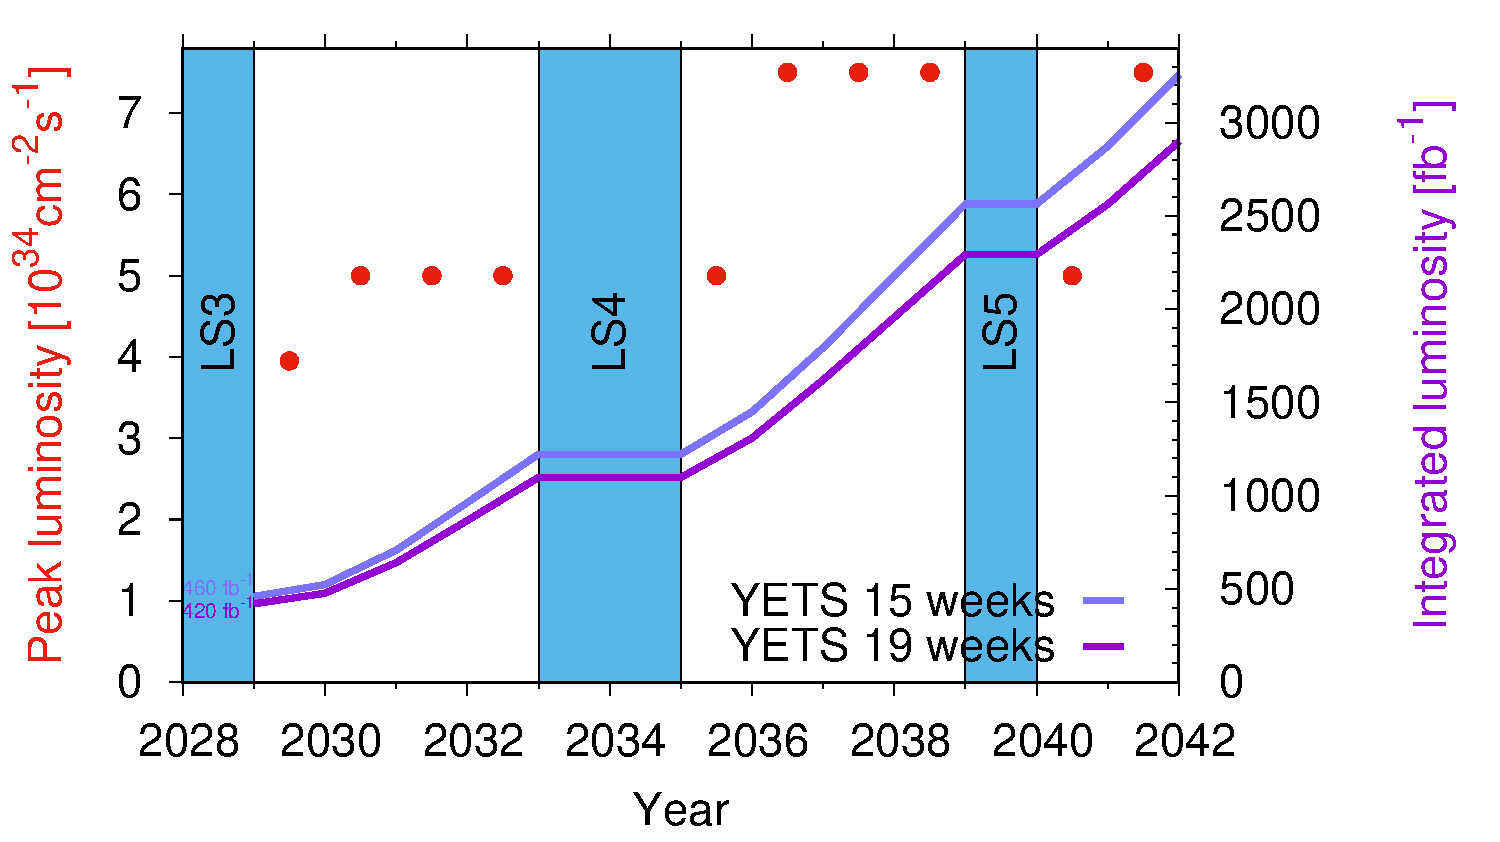
\includegraphics[width=0.8\textwidth]{figures/Part2/Upgrade/Lumi}
 \end{tabular}
 \caption{The peak and intergraded luminosity expected to be delivered by the \ac{HL-LHC}, taken from~\cite{LHC:plan} in November 2023. The left-hand $y$-axis shows the scale of the peak instantaneous luminosity, which is itself represented with red dots. The right-hand $y$-axis shows the scale of the intergraded luminosity. The two solid lines represent the intergraded luminosity under two \ac{YETS} scenarios.}
 \label{fig:Lumi}
 \end{center}
\end{figure}

An overview of the Phase-2 Upgrade is given in \autoref{sec:Overview}. Among various systems upgrades, the upgrade of the Outer Tracker is more relevant to this thesis, which is described in \autoref{sec:OT}. The Outer Tracker upgrade will enable tracking at the \ac{L1} trigger, which is discussed in \autoref{sec:Algo}. The tracking information can be combined with the calorimeter responses to build electron candidates at the \ac{L1} trigger, which is discussed in \autoref{sec:L1Ele}.

\section{Overview of the Upgrade}
\label{sec:Overview}

A new silicon tracker~\cite{CMS:2017lum} will replace the current tracker for the Phase-2. The Phase-2 tracker is divided into two subsystems: a pixel detector known as the Inner Tracker and the Outer Tracker composed of strip and macro-pixel sensors. Thanks to the extended coverage of the Inner Tracker, the Phase-2 Tracker will provide efficient tracking up to $|\eta|~<$ 4. The Phase-2 tracker is also much lighter with improved radiation hardness while enjoying a reduced material budget in the tracking volume. The granularity of the Phase-2 tracker will be increased by roughly a factor of 4, leading to a much better charged-particle $\pt$ resolution. More importantly, the Phase-2 Outer Tracker is specially designed to be capable of delivering data to the \ac{L1} trigger, which is further discussed in \autoref{sec:OT}.

The latency and event rate of the hardware-based \ac{L1} trigger will be increased (from 3.4 $\mu$s) to 12.5 $\mu$s and (from 100 kHz) 750 kHz, respectively, for the Phase-2~\cite{Zabi:2020gjd}. The increased latency leaves sufficient time for the track construction as well as correlating information from the tracker, calorimeters, and Muon system on \ac{L1} hardware. The addition of tracking information also enables the implementation of more sophisticated trigger algorithms at \ac{L1}, such as those based on the \ac{PF}~\cite{CMS:2017yfk} or \ac{PUPPI} algorithms~\cite{Bertolini:2014bba}.

The frontend electronics of the \ac{ECAL} Barrel Calorimeter will be replaced~\cite{ECAL:upgrade} to accommodate the latency and rate requirements of the Phase-2 \ac{L1} trigger, and to provide better timing resolution. The upgraded frontend electronics will enable the \ac{L1} trigger to exploit the information from single crystals as opposed to the trigger primitive of $5\times5$ crystals provided by the current system. The more granular trigger primitives will improve the precision of identifications and isolations of calorimeter objects and the matching between tracks and electromagnetic showers at \ac{L1}. 

The \ac{ECAL} and \ac{HCAL} Endcap Calorimeters will be replaced by a new endcap calorimeter known as the \ac{HGCAL}~\cite{CMS:2017jpq}. The \ac{HGCAL} is a sampling calorimeter consisting of both electromagnetic
and hadronic sections, which are designed to withstand the extreme radiation level at the \ac{HL-LHC}. It provides an excellent timing resolution and incorporates the concept of three-dimensional shower measurements from experiments at the \ac{ILC}~\cite{CALICE:2008kht}. Like both of its predecessors, the \ac{HGCAL} is designed to contribute to the \ac{L1} trigger.

A brand new subsystem known as the \ac{MTD}~\cite{Butler:2019rpu} will be added to the \ac{CMS} Phase-2 lineup. The \ac{MTD} covers both barrel and endcap regions and it enables the measurements of the production timing of the \acp{MIP}. This addition enables the four-dimensional reconstruction of the interaction vertices, which represents a completely new capability added to the \ac{CMS} detector. The timing information associated with the reconstructed vertices will provide a much-needed handle to cope with the high \ac{PU} conditions at the \ac{HL-LHC}.

As explained in \autoref{sec:MuonSys}, the \ac{CSC} in the endcap region will be complemented by a new subsystem \ac{GEM}, which is expected to be fully operational by \ac{LS} 3. Similar to the \ac{ECAL} Barrel, the electronics of the Muon system will also be upgraded to meet the \ac{L1} trigger requirements~\cite{Hebbeker:2017bix}.

Upgrades of the \ac{HLT} and \ac{BRIL} system are also planned and are documented in detail in Ref.~\cite{HLT:Upgrade} and~\cite{Beam:Upgrade}, respectively. 

\section{The Outer Tracker Upgrade}
\label{sec:OT}

The performance of the current \ac{CMS} Tracker will be significantly degraded if it continues to take data beyond the designed radiation exposure (500 fb$^{-1}$) in the \ac{HL-LHC} era. Therefore, it must be completely replaced by a new tracker by the end of Run-3, which is envisioned to be able to withstand radiation damage up to 3000 fb$^{-1}$. 

The design of the Phase-2 Outer Tracker is largely driven by the task of providing tracking information to the \ac{L1} trigger. The feasibility of a track trigger at \ac{L1} is significantly challenged by the sheer data volume generated by the \ac{HL-LHC} at a frequency of 40 MHz accompanied by up to 200 \ac{PU}. A novel tracker module design, known as the ``$\pt$ module''~\cite{Foudas:2005xf} is used to reduce the data volume effectively while keeping interesting events for physics analyses. Under this design, the Outer Tracker will be composed of over three thousand $\pt$ modules, and each consists of two closely spaced silicon sensors that are parallel to each other. Through correlating hits from the two parallel sensors, the $\pt$ modules are capable of providing $\pt$ discrimination, thus reducing the data volume at the front end. Correlated pairs of hits are referred to as ``stubs'', which serve as the trigger primitive to the \ac{L1} trigger. The stub mechanism is illustrated in Figure~\ref{fig:Stub}. With the current design, only hits over the threshold of 2 GeV will be read out, which corresponds to a data reduction rate of up to 100.

\begin{figure}[tbh!]
 \begin{center}
 \begin{tabular}{cc}
  \centering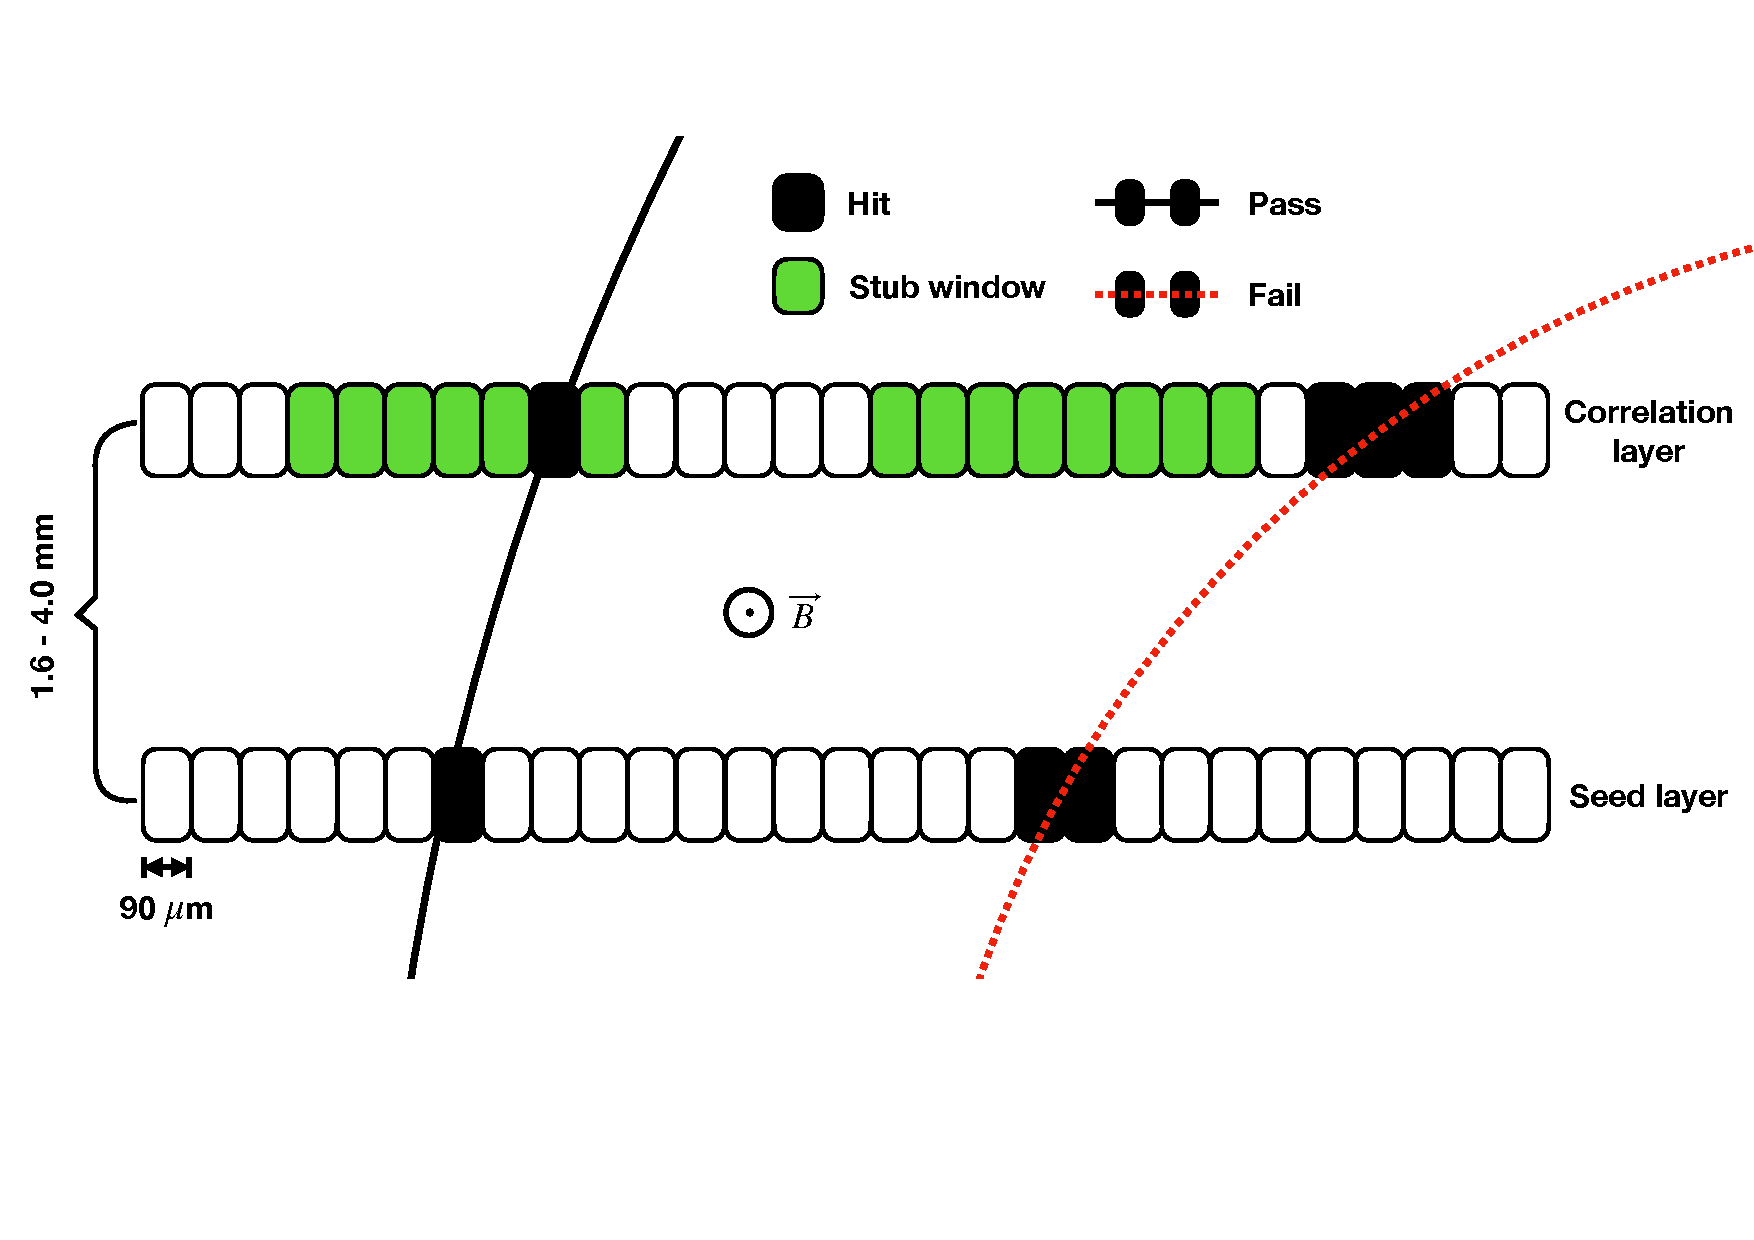
\includegraphics[width=0.9\linewidth]{figures/Part2/Upgrade/Stub}
 \end{tabular}
 \caption{Illustration of the stub mechanism in a cross-sectional view of a $\pt$ module (2S) in the magnetic field. Charged particles with a $\pt$ higher than 2 GeV are represented with the black solid curve while the red dashed curve represents charge particles with lower $\pt$. The magnetic field will cause low $\pt$ charged particles to bend with a smaller radius of curvature, and thus fail the pre-determined stub window corresponding to a $\pt$ threshold of 2 GeV.}
 \label{fig:Stub}
 \end{center}
\end{figure}

The Phase-2 Outer Tracker consists of six cylindrical barrel layers (L1-L6) and five disks (D1-D5) on each side of the endcap, as illustrated in \ref{fig:TrackerGeo}. The layers and disks of the Outer Tracker are composed of two types of $\pt$ modules, known as the ``Pixel-Strip (PS)'' modules and ``Strip-Strip (2S)'' modules. Sketches of the PS and 2S modules are shown in Figure~\ref{fig:Modules}. The PS modules occupy the first three barrel layers as well as regions of the disks that are closer to the beam line. The remaining regions of the disks as well as the last three barrel layers are occupied by the 2S modules. The Outer Tracker layout shown in figure~\ref{fig:TrackerGeo} is known as the so-called ``tilted geometry'' where the PS modules in the barrel layers are positioned with various titled angles to increase the stub efficiency.

\begin{figure}[tbh!]
 \begin{center}
 \begin{tabular}{c}
  \centering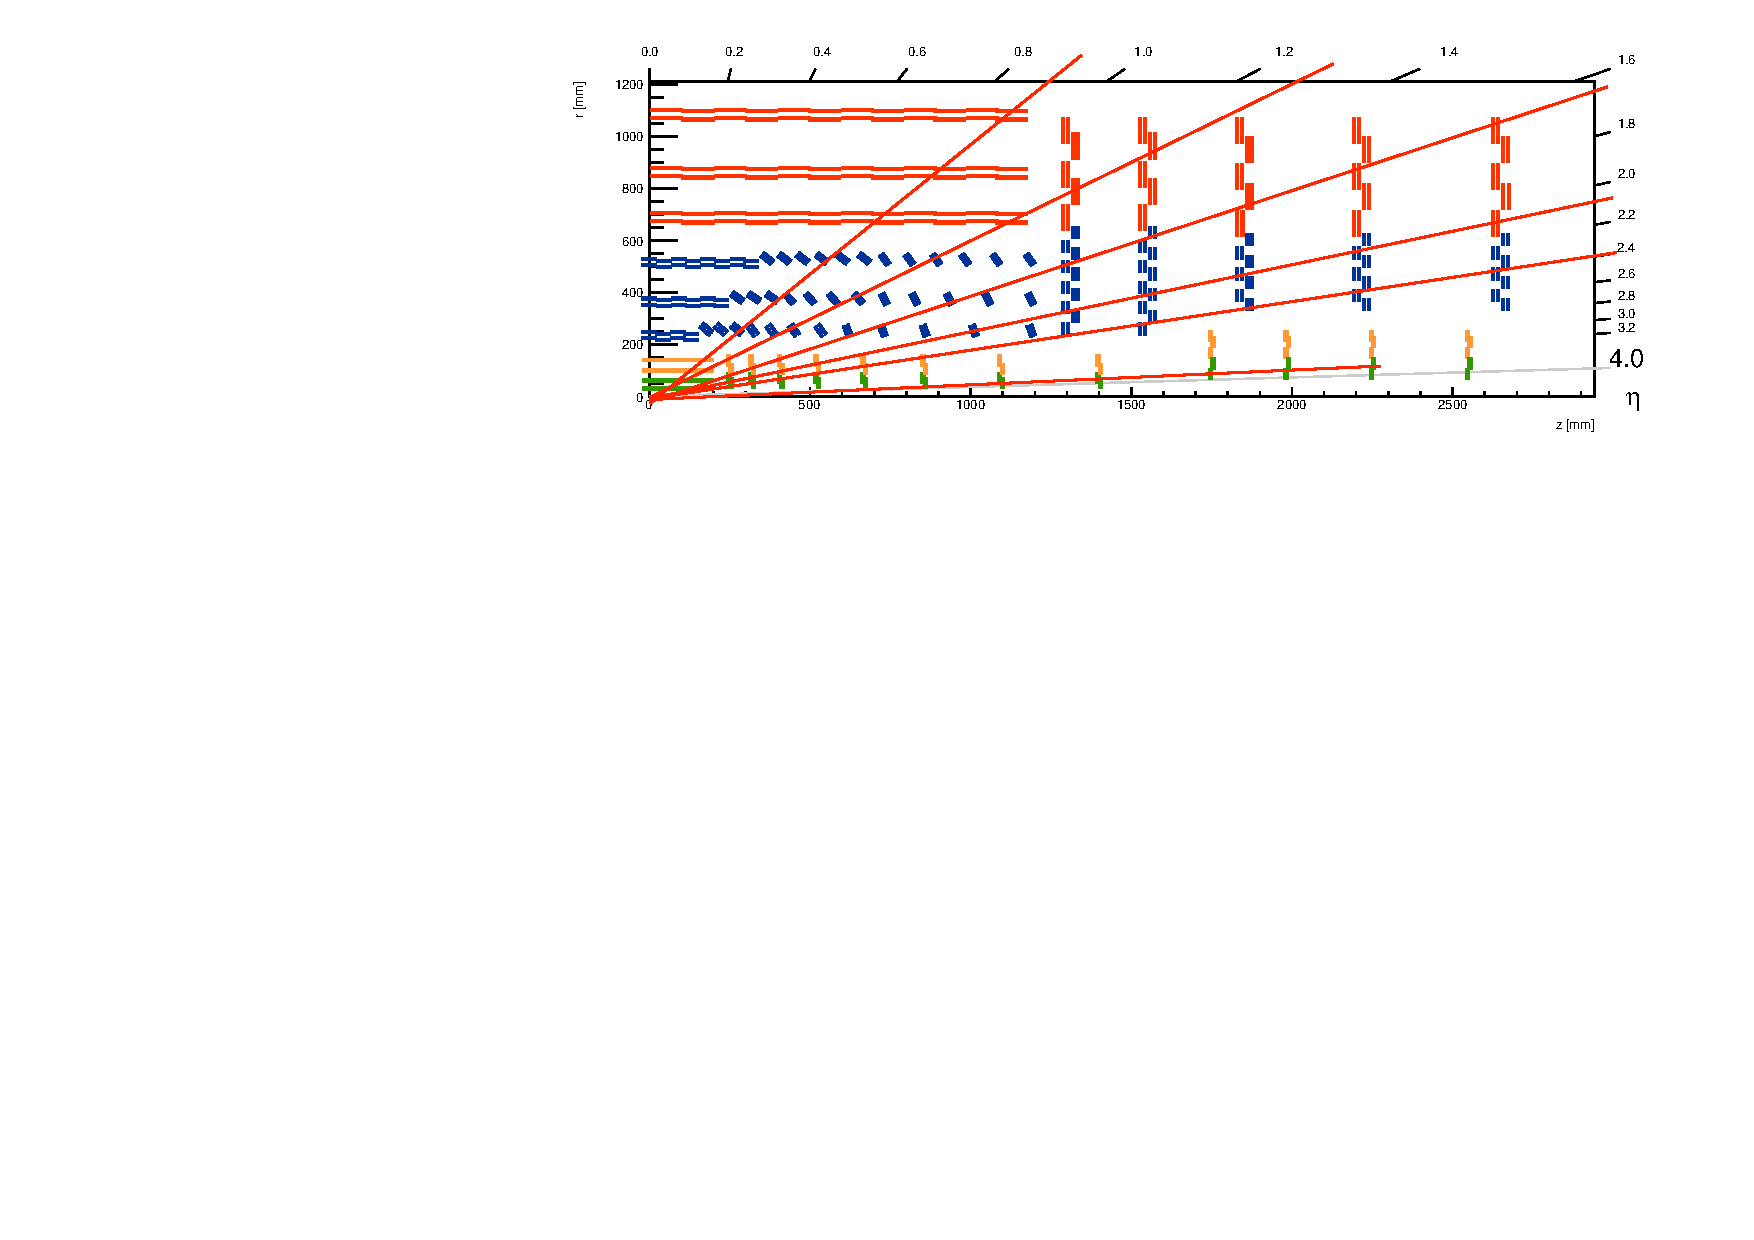
\includegraphics[width=0.9\linewidth]{figures/Part2/Upgrade/TrackerGeo}
 \end{tabular}
 \caption{Layout of one quadrant of the Phase-2 \ac{CMS} tracker in the $r-z$ plane, generated by the \ac{CMSSW}~\cite{cmssw}. The PS modules of the Outer Tracker are represented with blue lines while the 2S modules are represented with red lines. The radial region below 200 mm is occupied by the Inner Tracker, whose modules are represented with orange and green lines. The Inner Tracker does not contribute to the \ac{L1} trigger.}
 \label{fig:TrackerGeo}
 \end{center}
\end{figure}

\begin{figure}[tbh!]
 \begin{center}
 \begin{tabular}{c}
  \centering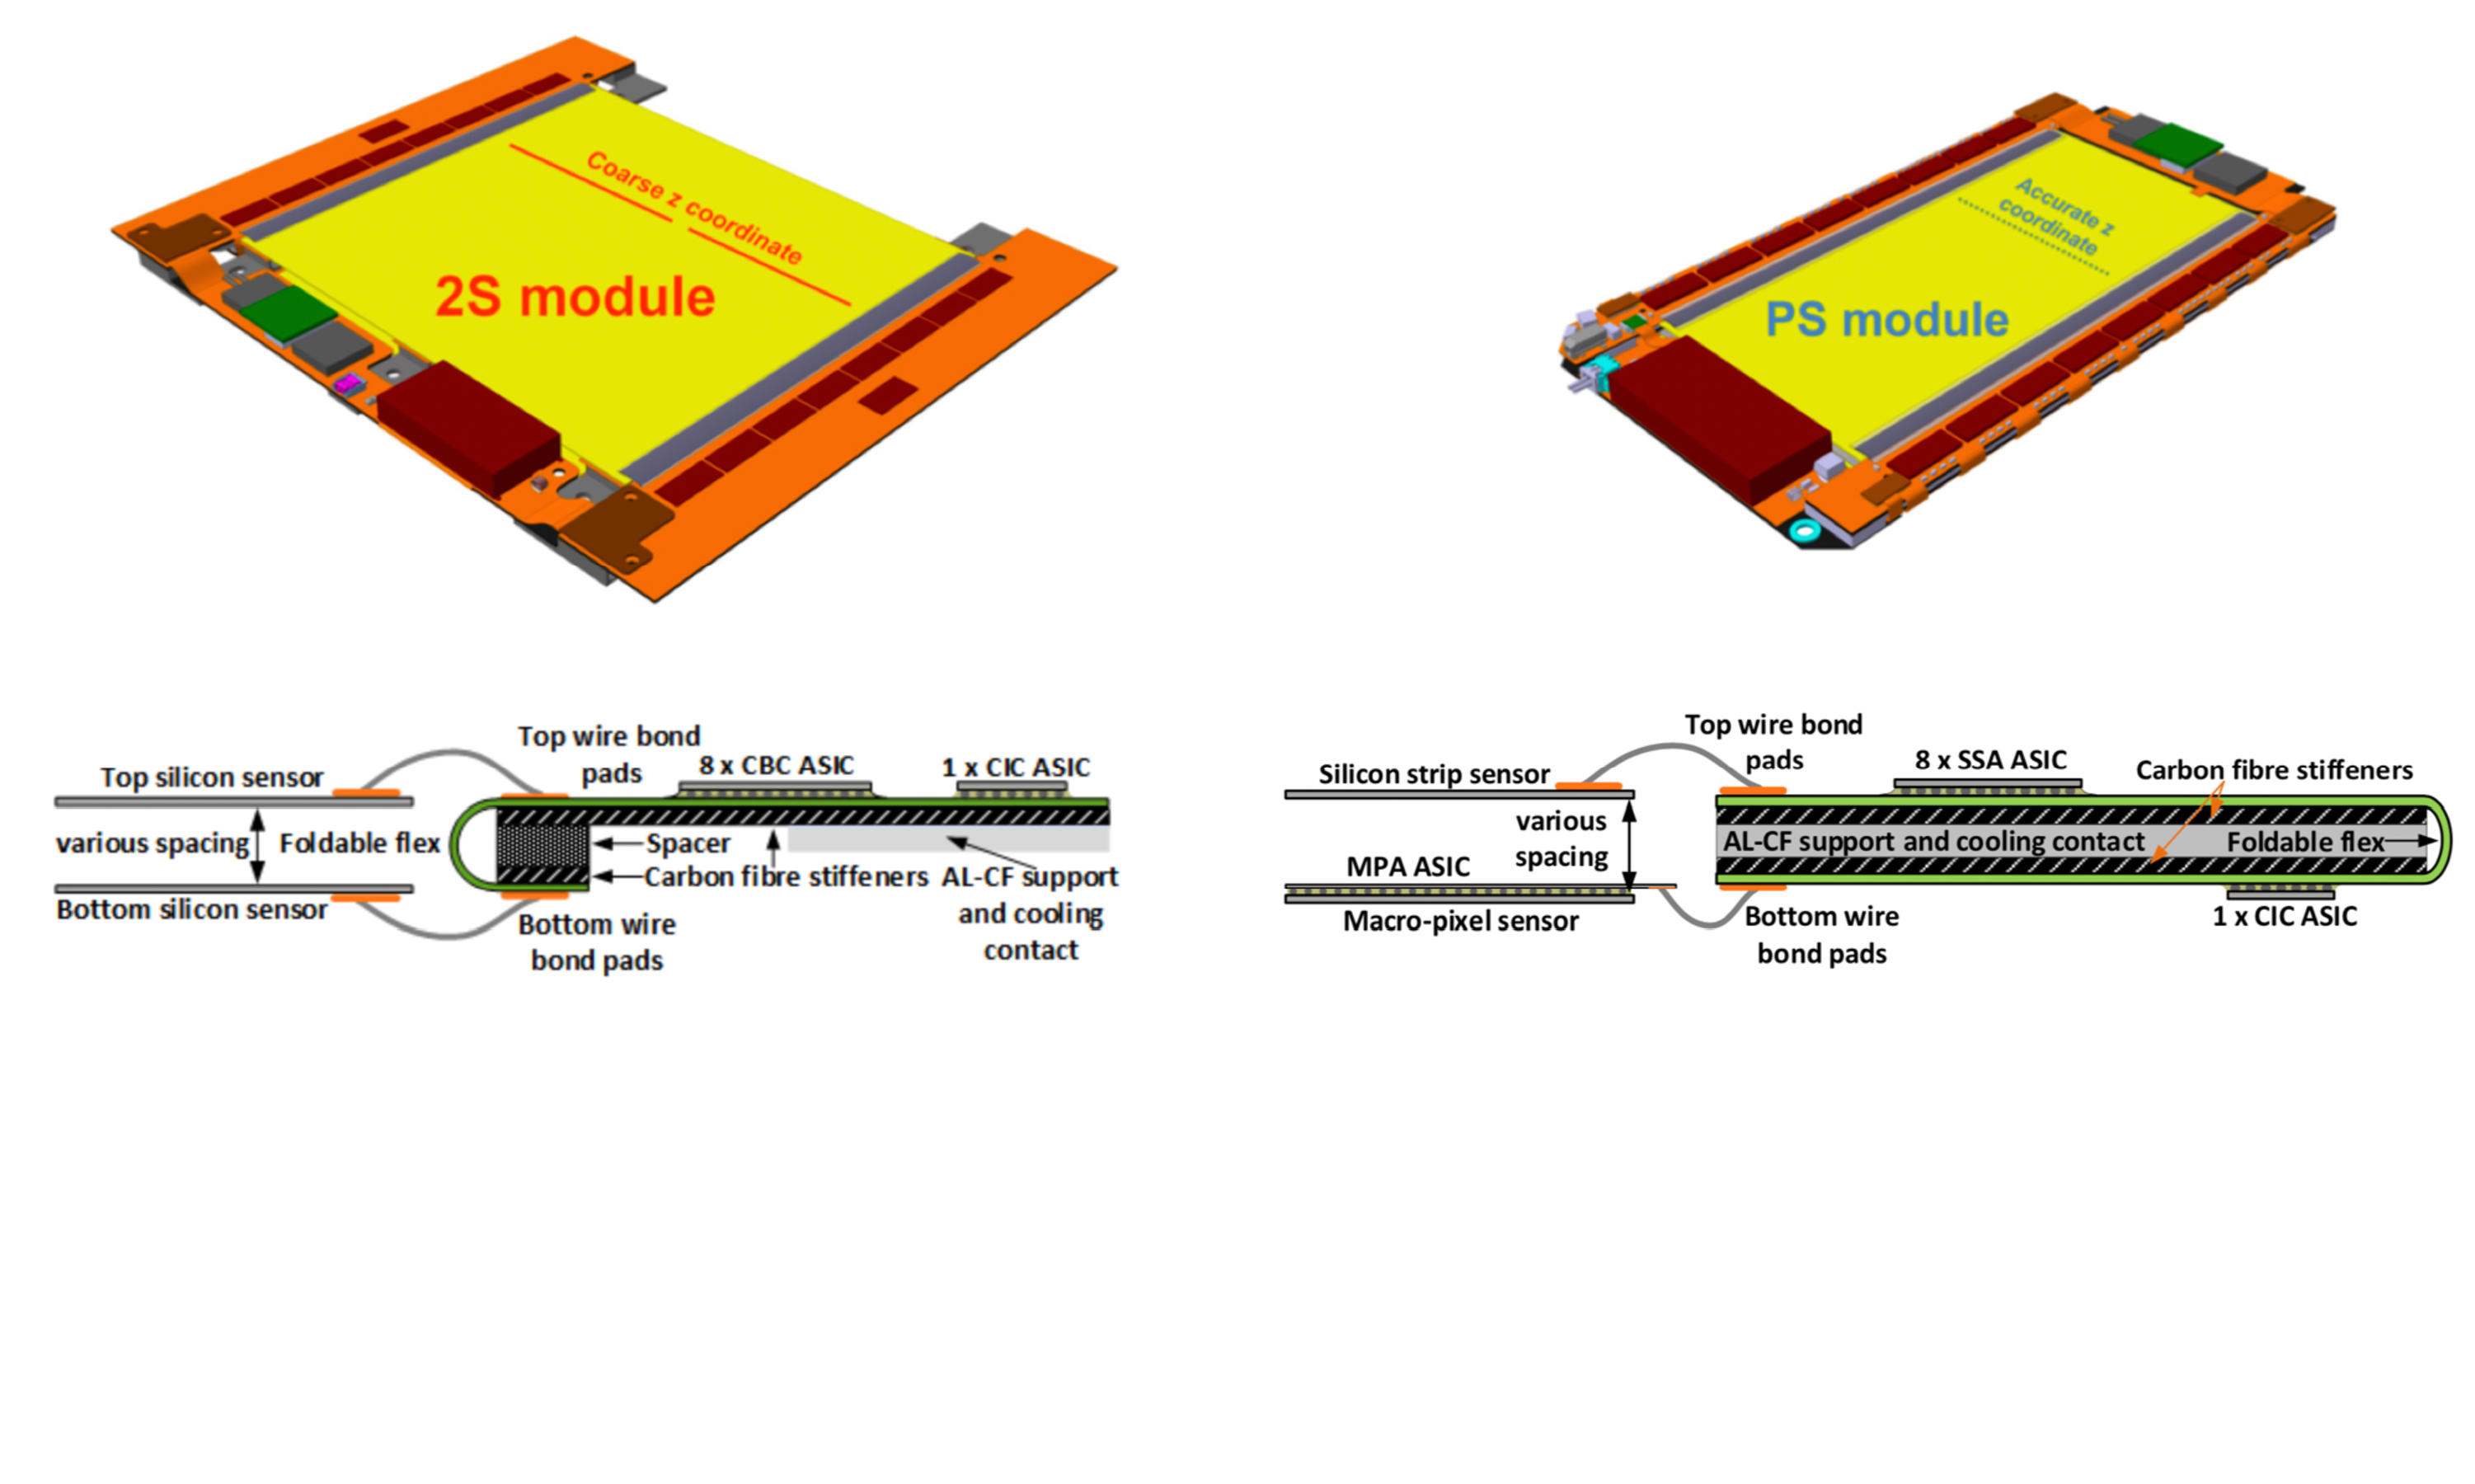
\includegraphics[width=0.95\linewidth]{figures/Part2/Upgrade/Modules}
 \end{tabular}
 \caption{Illustrations of the 2S module (left) and PS module (right), adapted from~\cite{CMS:2017lum}. Shown are views of the assembled modules (top) and sketches of the connection between frontend hybrids and silicon sensors (bottom).}
 \label{fig:Modules}
 \end{center}
\end{figure}

The 2S module consists of two 90 cm$^{2}$ strip sensors separated by a few millimeters using a \ac{Al-CF} spacer. Each strip sensor consists of over two thousand strips arranged in two rows. Each strip is 5 cm long with a pitch of 90 $\mu$m. The two sensors are connected to hybrid circuits known as the frontend hybrid and service hybrid. The frontend hybrid consists of eight \ac{CBC}~\cite{Raymond:2012zz}, which is responsible for readout. The service hybrid is mainly responsible for powering.

The PS module is about half the size of the 2S module in its active area. It has one strip sensor on the top and one macro-pixel sensor on the bottom, which provides very precise measurements of $z$-coordinates. Similar to the 2S module, the strip sensor of the PS module consists of roughly two thousand strips. Each strip is about 2.4 cm long with a pitch of 100 $\mu$m. The macro-pixel sensor contains 960 $\times$ 32 macro-pixels with a length and pitch of 1.5 cm and 100 $\mu$m, respectively. The two sensors are connected to hybrid circuits that are responsible for readout~\cite{Ceresa:2016mqm} and powering.

\section{Level-1 Track Finder}
\label{sec:Algo}

The task for track finding algorithms at \ac{L1} can be broken down into two main parts: i) performing pattern recognition to identify and correlate all possible stubs that belong to the same charged particle trajectory and ii) obtaining the parameters of the trajectory by fitting the reconstructed tracks. A latency of roughly 4 $\mu$s is allocated to track finding algorithms, which becomes one of the critical constraints in algorithm development. Multiple approaches~\cite{CMS:2017lum} have demonstrated the feasibility of delivering tracking information within the allowed latency and a so-called ``hybrid'' approach~\cite{Zabi:2020gjd} is adopted by \ac{CMS} as the way forward.

To meet the latency requirement and increase redundancy, the hybrid approach is parallelized both in space and in time. The Outer Tracker is partitioned into nine $\phi$ sectors and stubs in each sector are processed in parallel with a time-multiplexing factor of 18. The main stages of the hybrid approach are similar to the offline \ac{CTF} algorithm described in \autoref{sec:Track}, including seeding, pattern recognition, and parameter fitting, as illustrated in Figure~\ref{fig:algorithm}. The main difference is that the parameter fitting is disentangled from the pattern recognition in the hybrid approach while these two stages are intergraded in the \ac{CTF} algorithm.

\begin{figure}[tbh!]
 \begin{center}
 \begin{tabular}{cc}
  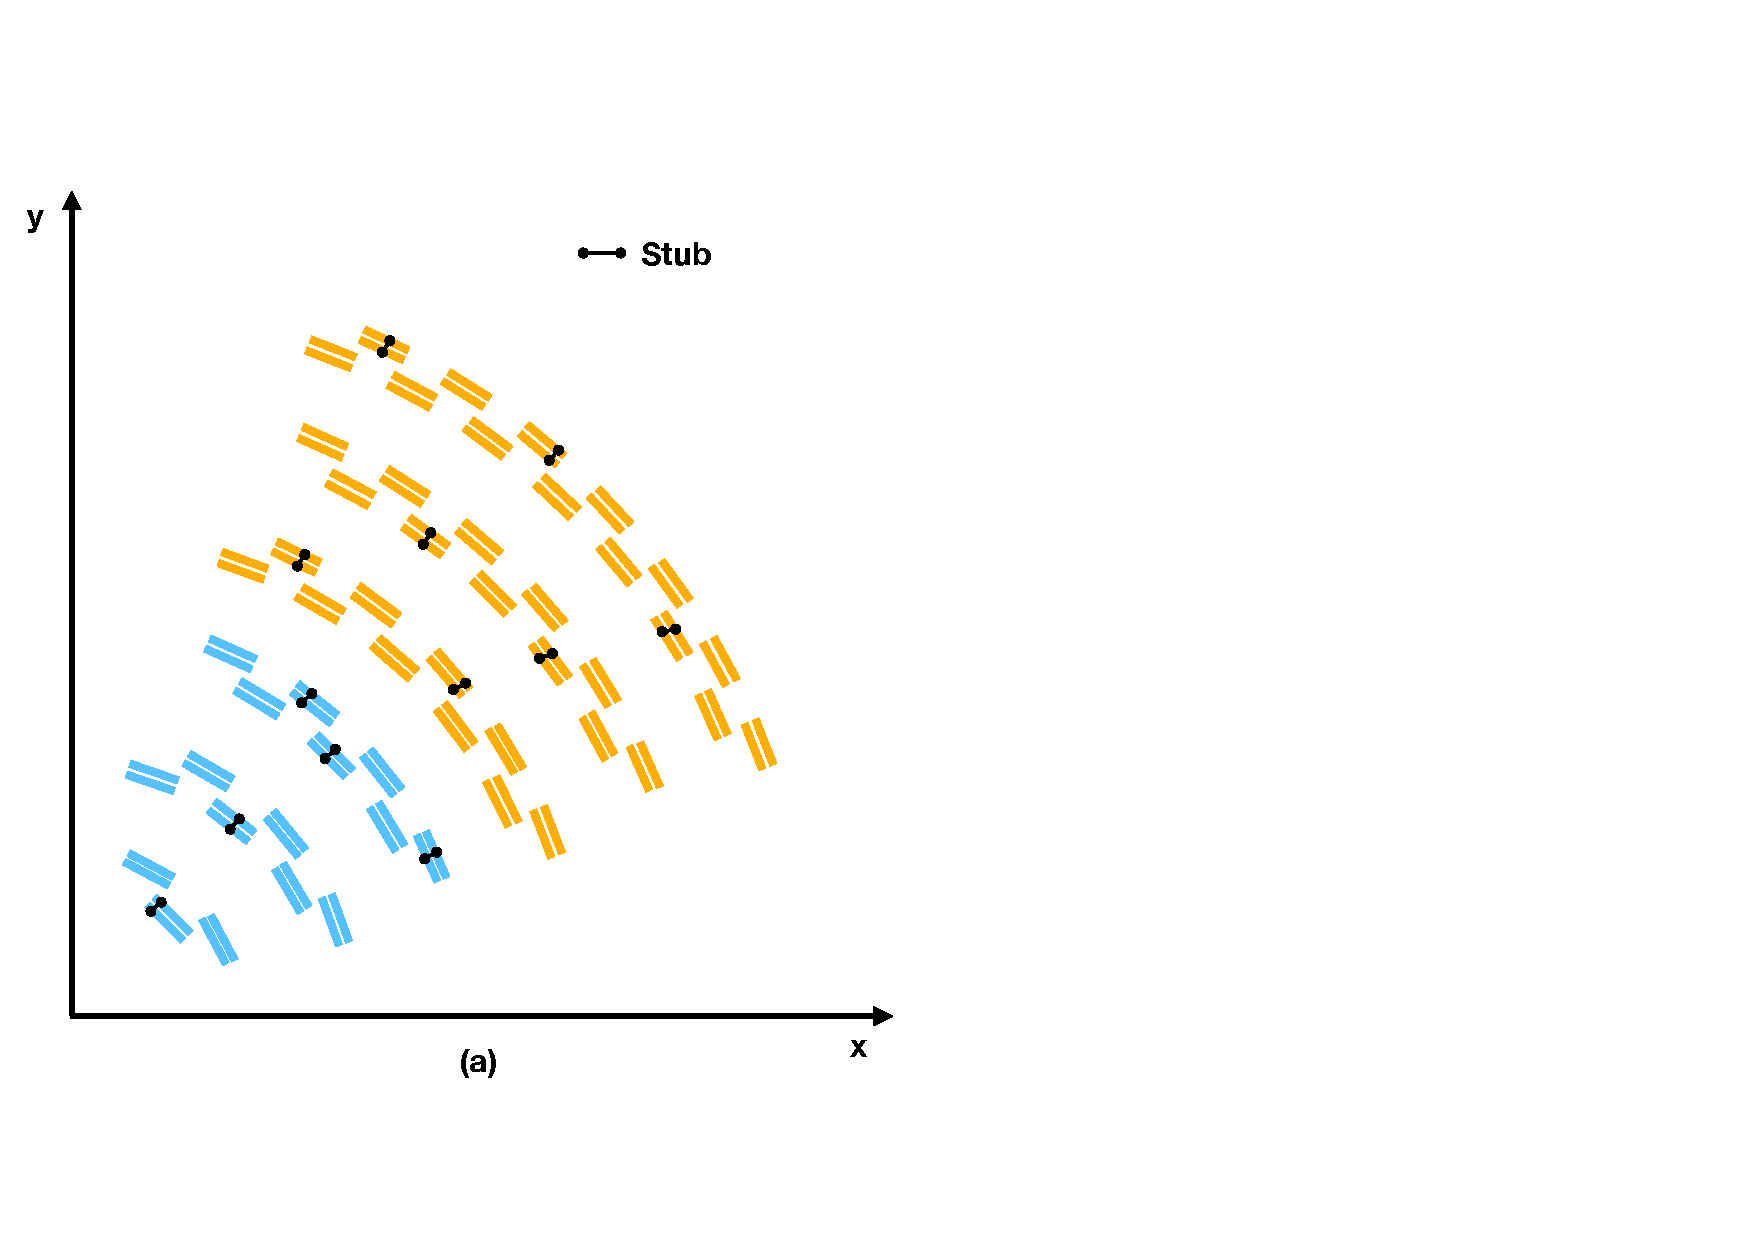
\includegraphics[width=.45\linewidth]{figures/Part2/Upgrade/tracklet1} &
  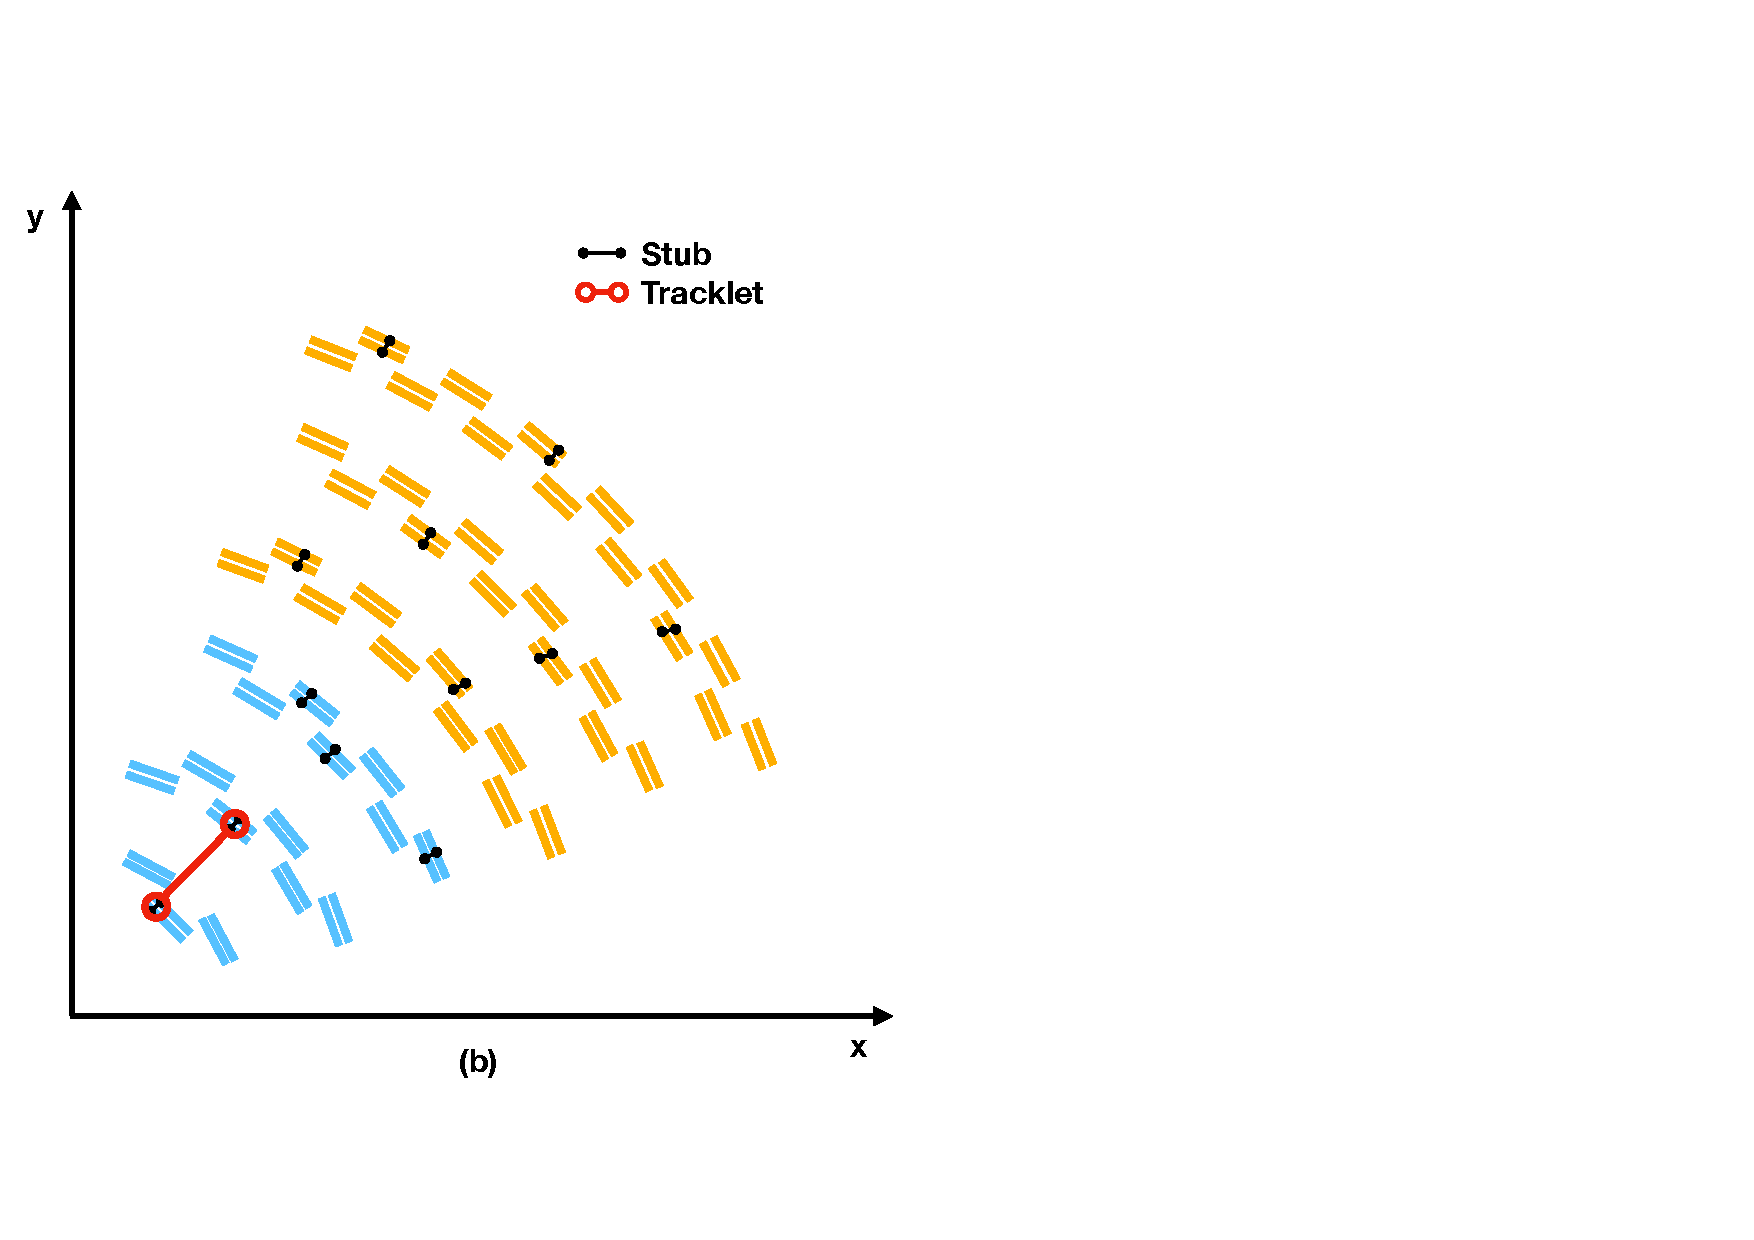
\includegraphics[width=.45\linewidth]{figures/Part2/Upgrade/tracklet2} \\
  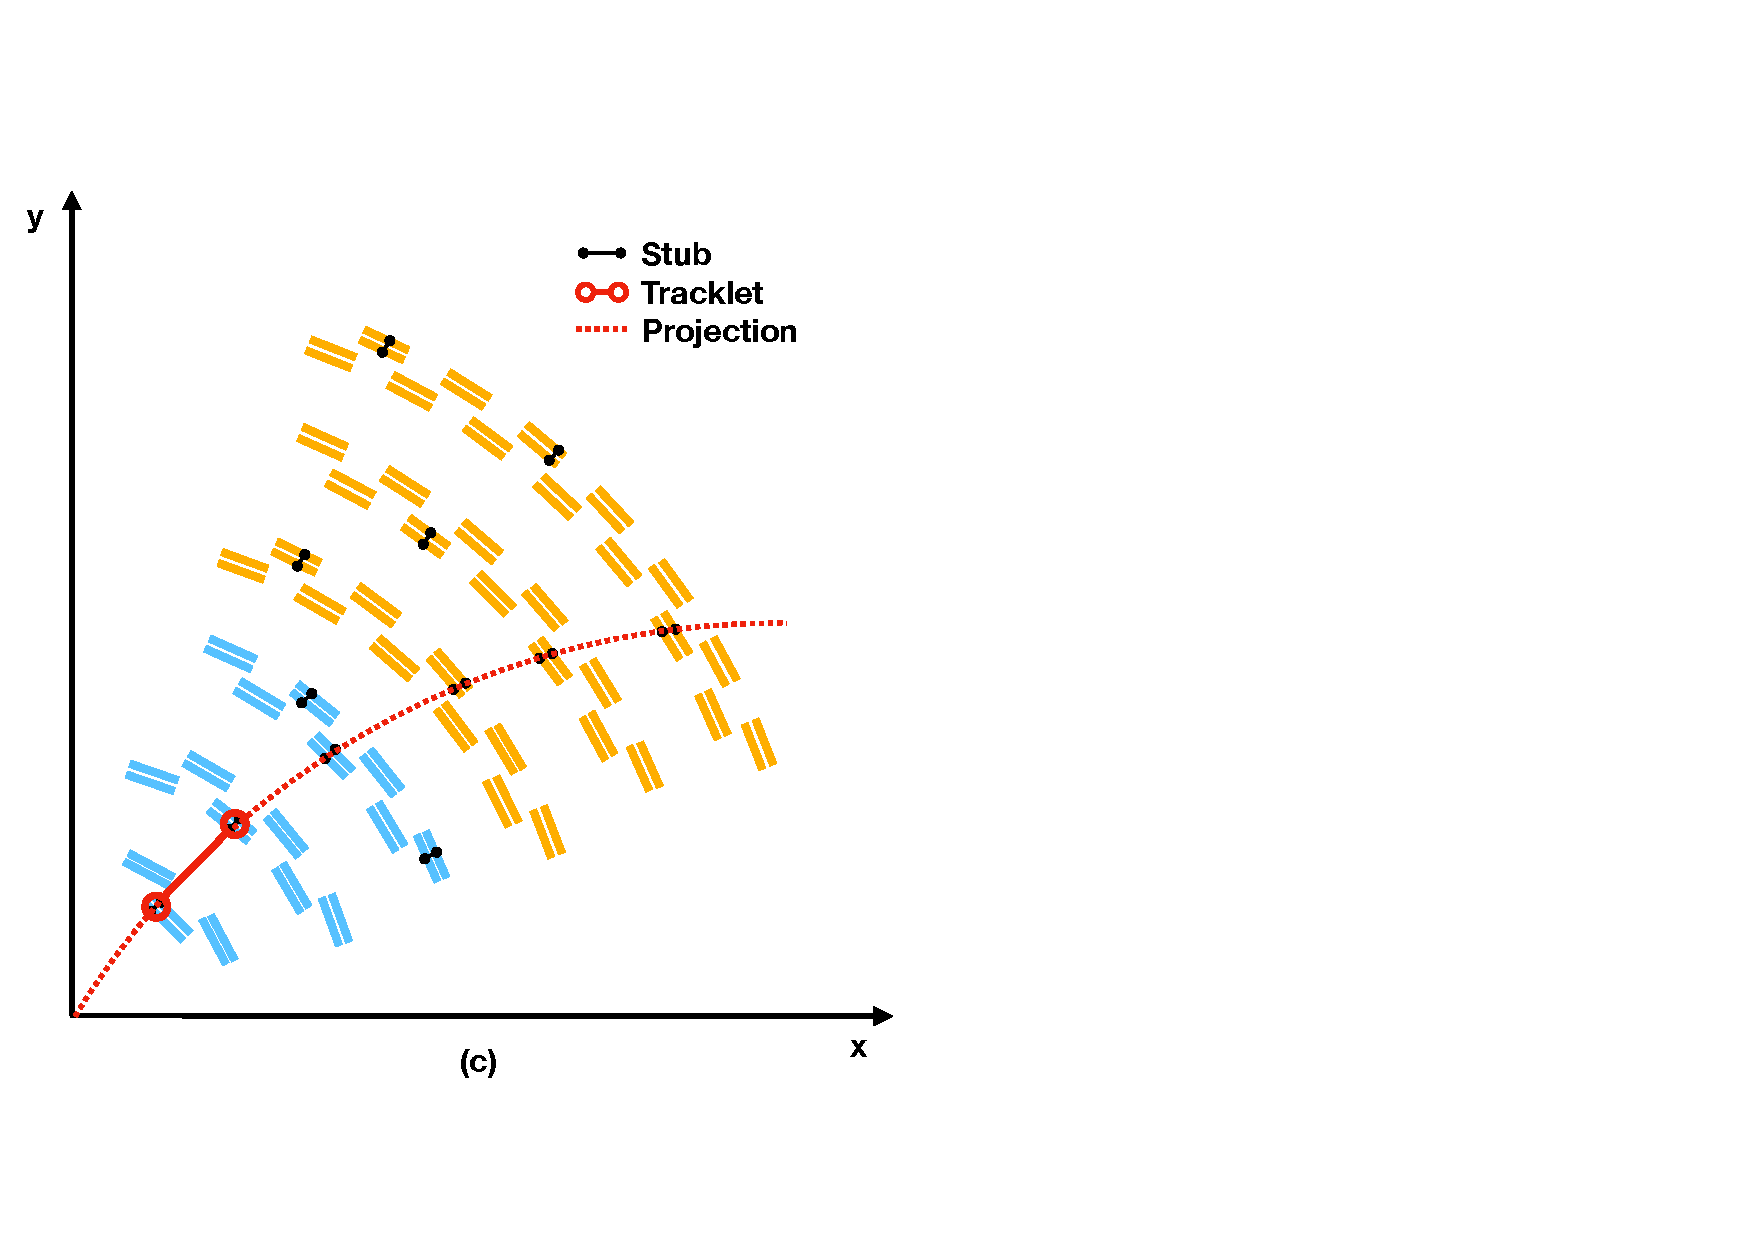
\includegraphics[width=.45\linewidth]{figures/Part2/Upgrade/tracklet3} &
  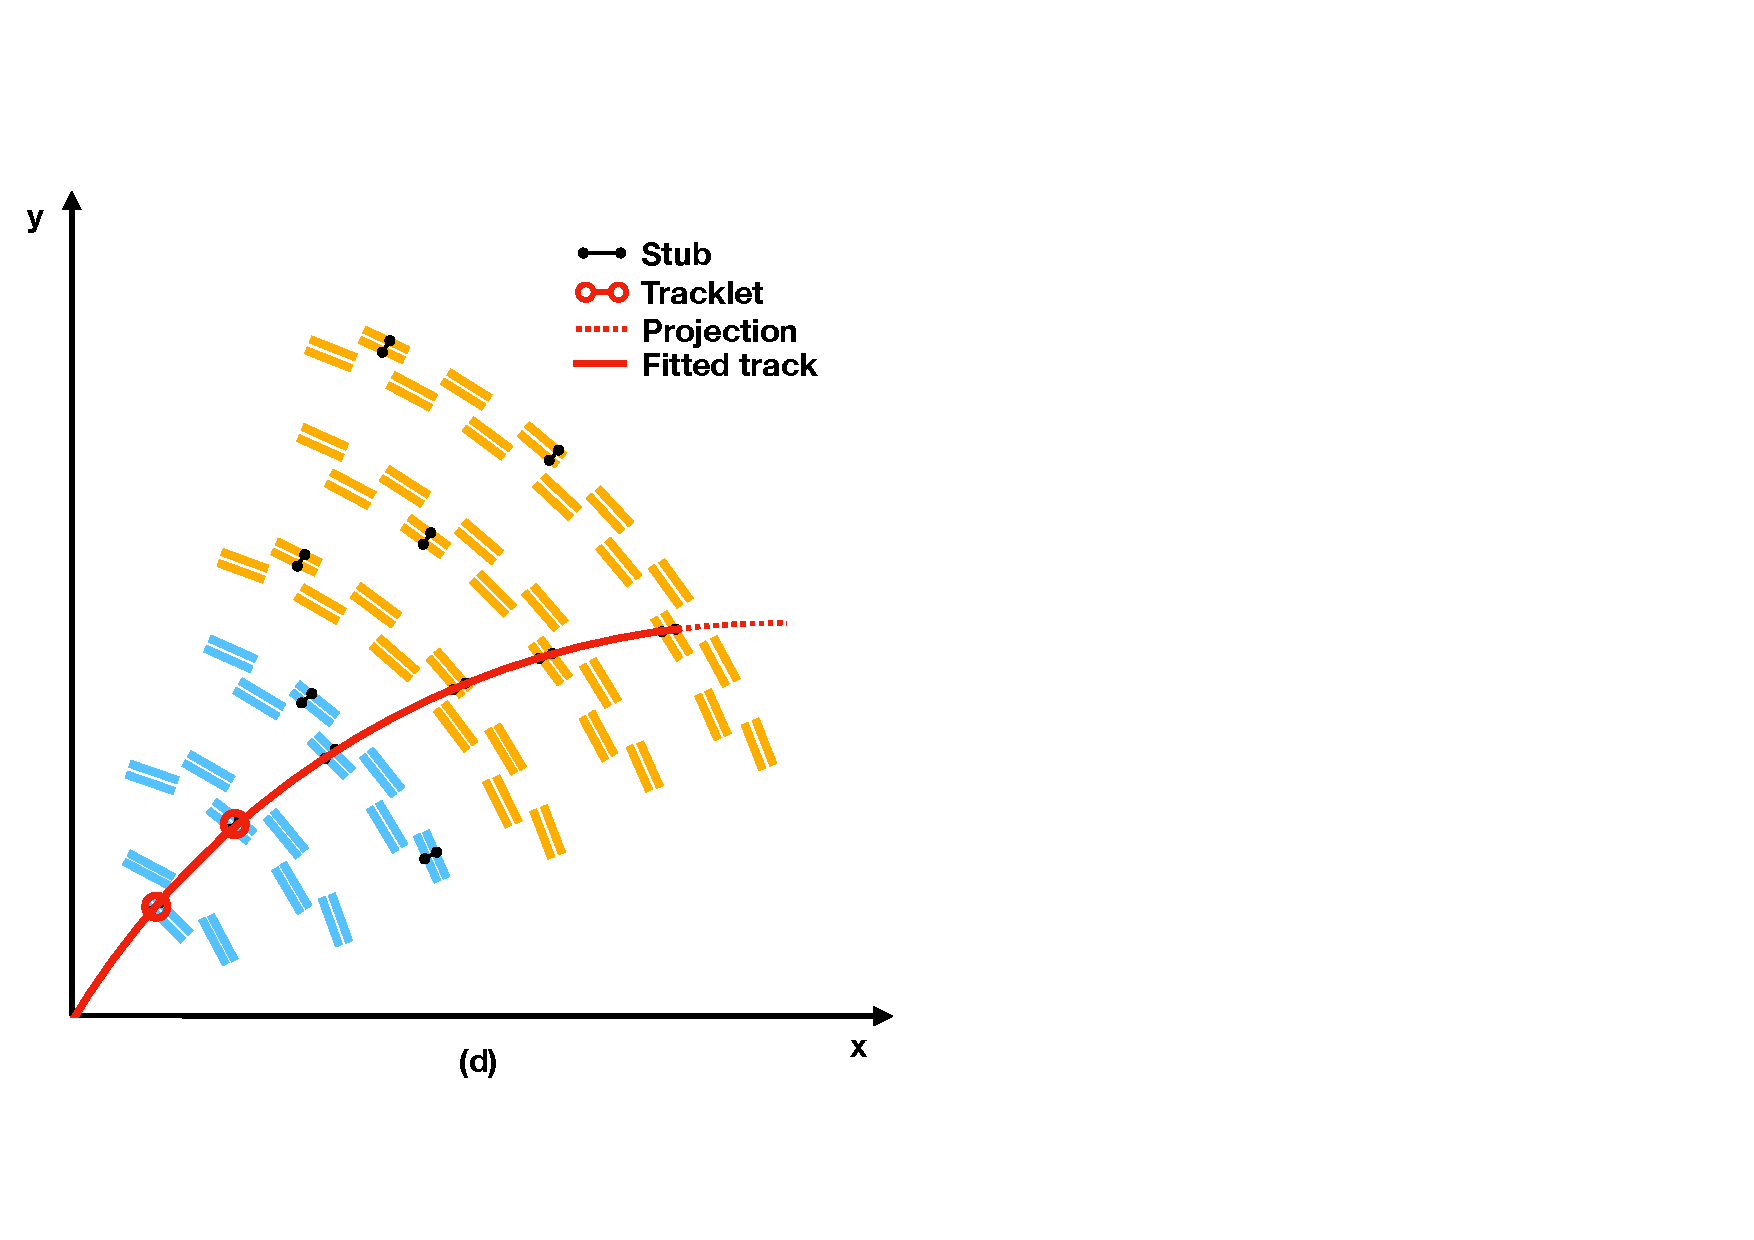
\includegraphics[width=.45\linewidth]{figures/Part2/Upgrade/tracklet4} \\
 \end{tabular}
 \caption{Illustration of different stages of the hybrid approach: (a) constructing stubs, (b) forming tracklet by correlating two stubs and the beam spot (origin), (c) projecting to other layers and finding matches, and (d) fitting track parameters using a \ac{KF}.}
 \label{fig:algorithm}
 \end{center}
\end{figure}

The initial stage of the hybrid approach involves correlating two stubs from two different Outer Tracker layers or disks under the assumption that trajectories of the charged particles originate from the beam spot. The correlated pair of stubs is referred to as the ``tracklet'' which is later used as a seed for the pattern recognition. The tracklet also comes with coarse parameter estimates which will be updated in the fitting stage. Seven combinations of layers/disks are attempted in parallel for seeding: L1+L2, L3+L4, L5+L6, D1+D2, D3+D4, L1+D1, and L2+D1. 

Based on its initial parameters, the tracklet is then extrapolated inward and outward to all possible layers or disks in parallel to look for stubs that belong to the same trajectory. A match is declared if a stub is found within a predetermined window around the projection in a layer or disk. At least two matches are needed in order to proceed to the following stage. 

Duplicates of the same track are produced as a result of the highly parallelized approach. Duplicated tracks are typically produced by two adjacent $\phi$ sectors when a charged particle is located near the sector boundary. Alternatively, they can be tracks that belong to the same sector but are seeded by different layer/disk combinations. To remove duplicates, tracks that share common stubs will be merged before the parameter fitting. 

The fitting stage is done by a \ac{KF} module that possesses the initial track parameters and adds stubs iteratively to update the track parameters. Each time a new stub is added, the consistency between the existing track parameters and the new stub will be checked which provides input to the parameter update. All potential combinations of stubs are attempted by the \ac{KF}, and the final residual of each combination is calculated and compared. The stub combination with the best residual is finally chosen as the \ac{KF} output. 

Tracks coming out of the fitting stage are considered to be the final product since all the track parameters are final. Similar to the offline track finder discussed in \ref{sec:Track}, fake tracks can still be reconstructed by the \ac{L1} track finder due to a variety of constraints and limitations of the algorithm. An additional module, referred to as the ``track quality'' is added to help distinguish, in a \ac{MVA} approach, between genuine tracks that can be associated with charged particles and fake tracks. A score between 0 and 1 is calculated for each track by combining multiple variables, such as the residuals produced by the \ac{KF}, into a \ac{BDT}. The score assigned to each track roughly translates to the probability of this track being genuine.

The hybrid track-finding algorithm has demonstrated a robust performance in software simulation, as shown in Figure~\ref{fig:trackingperformance}. The baseline version of this algorithm requires stubs from at least four unique layers and constrains the origin of the trajectories to the beam spot. An ``extended'' version of the algorithm is also in development, in which the beam spot constraint is relaxed. The extended tracking is especially useful in scenarios where tracks originate with a small displacement in the transverse plane, such as displaced electrons as a result of bremsstrahlung in the Inner Tracker. It has been shown that sizable improvement in electron tracking efficiency can be achieved by the extended tracking algorithm, as shown in Figure~\ref{fig:electronperformance}.

 \begin{figure}[tbh!]
 \begin{center}
 \begin{tabular}{cc}
  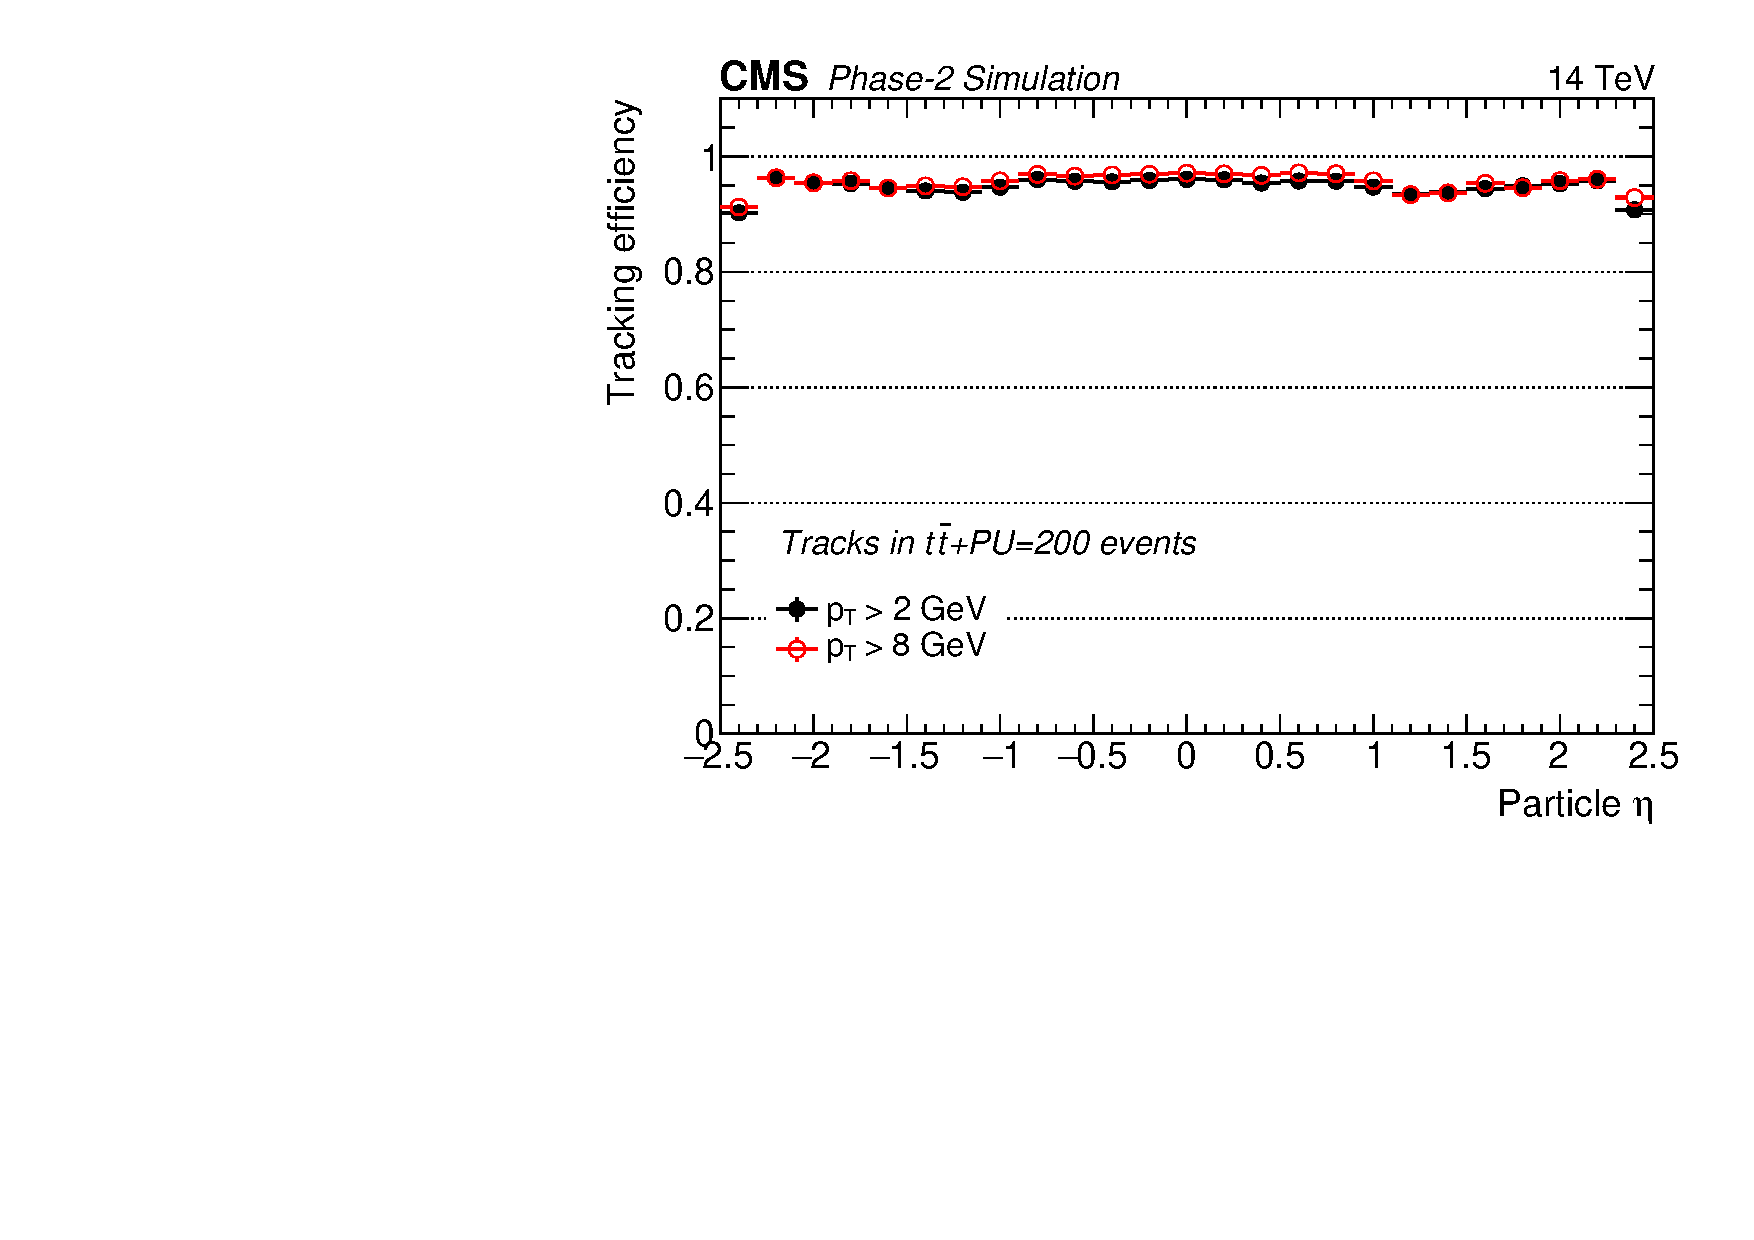
\includegraphics[width=.45\linewidth]{figures/Part2/Upgrade/L1TK_ttbar-pu200_eff_eta}&
  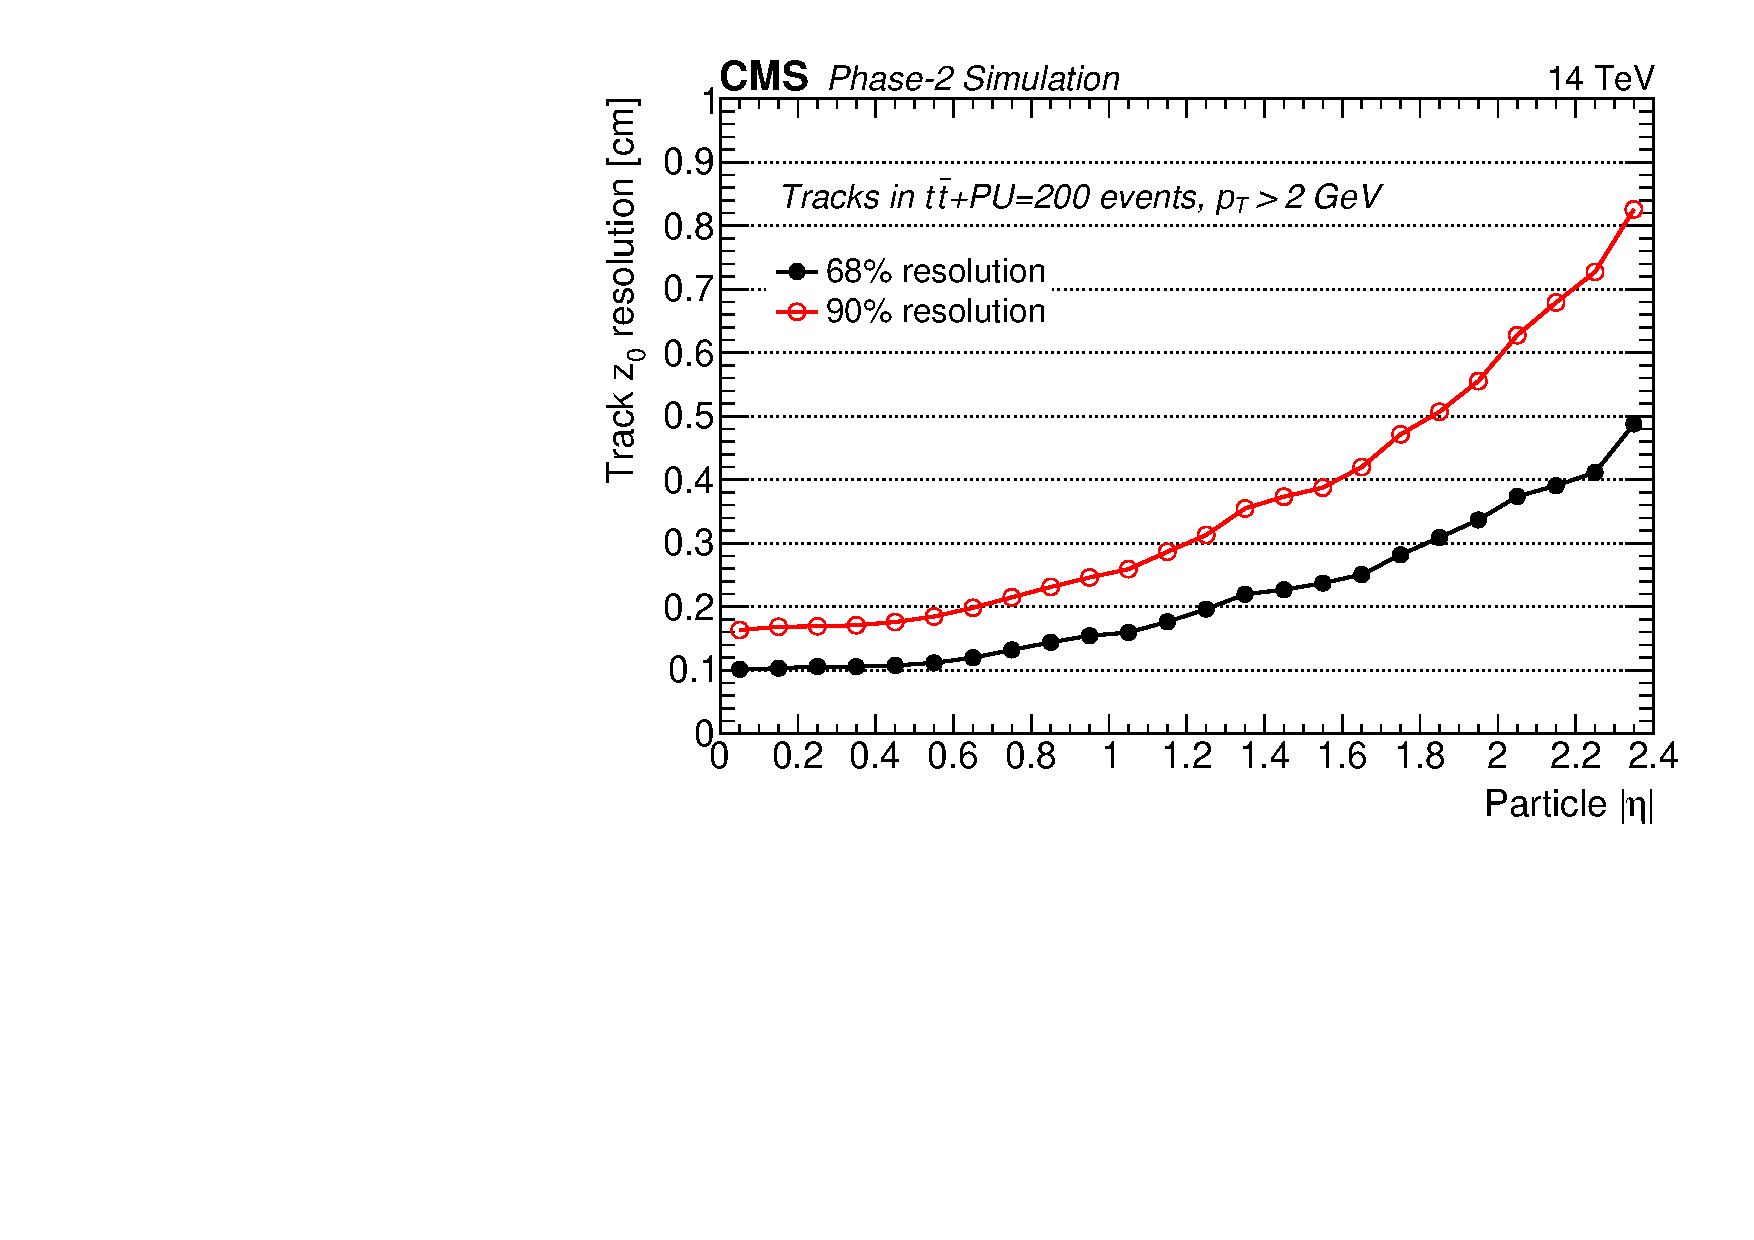
\includegraphics[width=.45\linewidth]{figures/Part2/Upgrade/L1TK_ttbar-pu200_resVsEta_z0}
 \end{tabular}
 \caption{(Tracking efficiency vs particle $\eta$, measured in $\ttbar$ samples (left). Track $z_0$ resolution vs particle $\eta$ (right).}
 \label{fig:trackingperformance}
 \end{center}
\end{figure} 

 \begin{figure}[tbh!]
 \begin{center}
 \begin{tabular}{cc}
  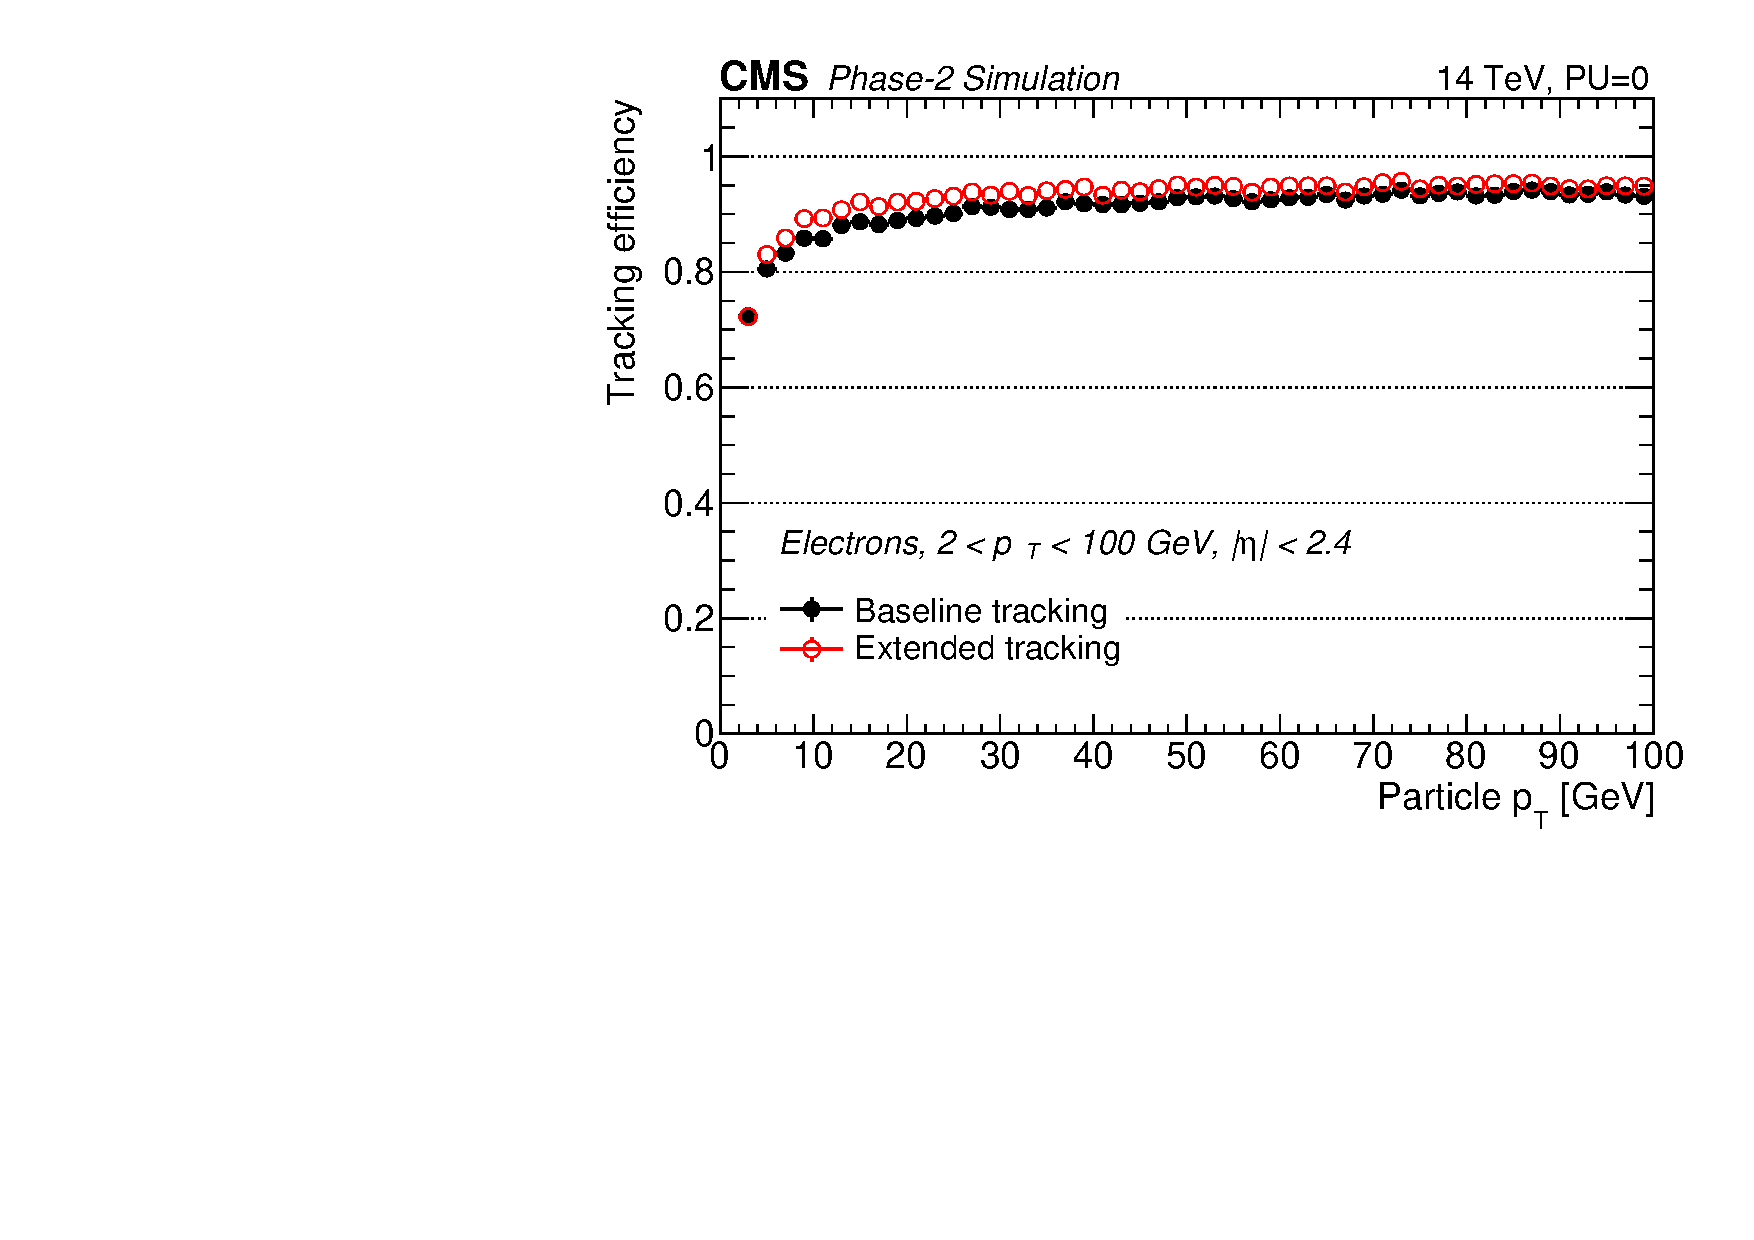
\includegraphics[width=.45\linewidth]{figures/Part2/Upgrade/L1TK_elec-pu0_eff_pt}&
  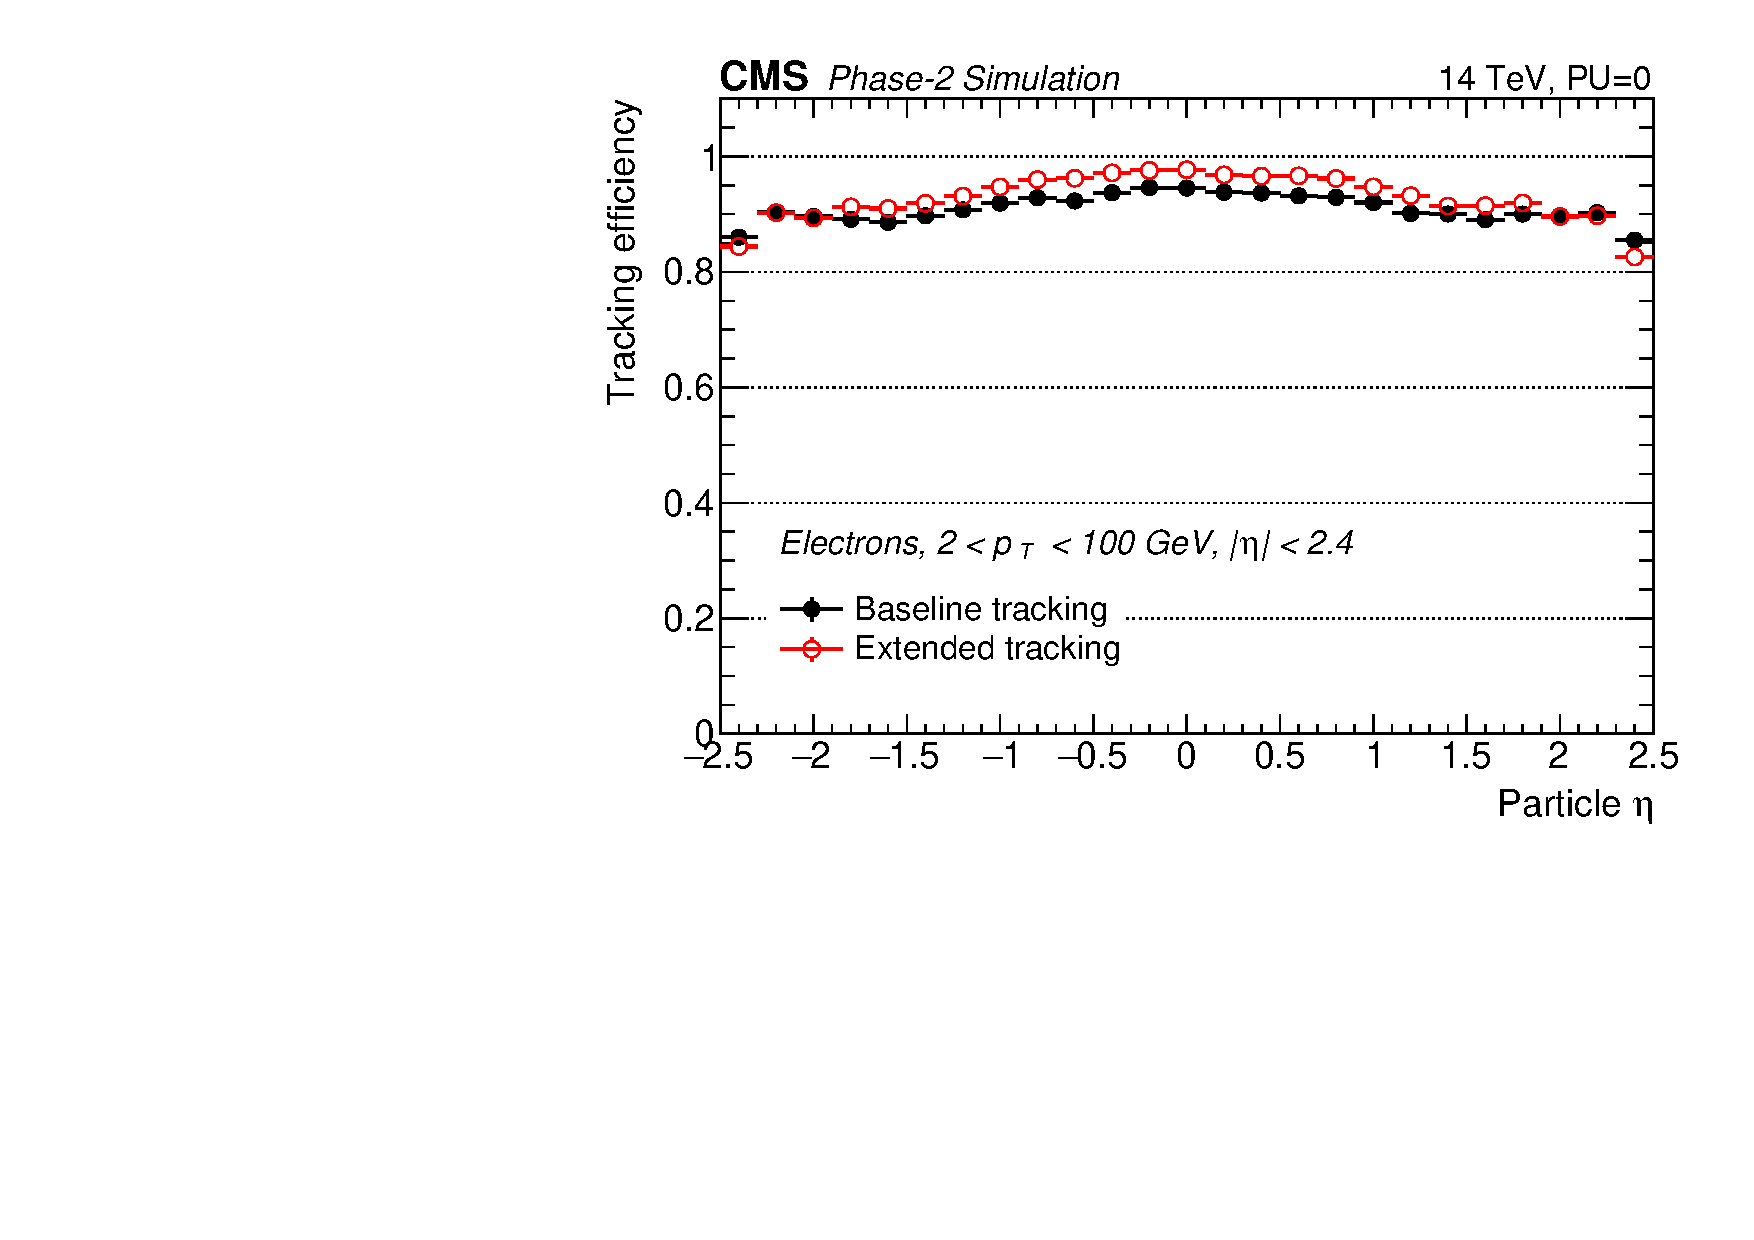
\includegraphics[width=.45\linewidth]{figures/Part2/Upgrade/L1TK_elec-pu0_eff_eta}
 \end{tabular}
 \caption{(Electron tracking efficiency vs particle $\pt$ (left) and $\eta$ (right), measured in simulated electron samples with 0 \ac{PU}.}
 \label{fig:electronperformance}
 \end{center}
\end{figure} 

\section{Level-1 Electron Trigger Algorithm}
\label{sec:L1Ele}

With the increase of the instantaneous luminosity, triggering on electrons at \ac{L1} will face unprecedented challenges as the data volume generated in the calorimeters becomes too large for the legacy trigger algorithms. The addition of tracking information provides a much-needed handle for the electron trigger. It enables precise track-calorimeter shower matching to control the trigger rate. To take advantage of this new tool, a new electron trigger algorithm is developed and documented in Ref.~\cite{Zabi:2020gjd}. 

The central feature of this algorithm is the fine-tuned matching between tracks produced by the \ac{L1} track finder and calorimeter clusters reconstructed in the \ac{ECAL} Barrel or \ac{HGCAL}. The baseline version of this algorithm extrapolates tracks to the calorimeter surface using the track $\pt$ and matches them with calorimeter clusters. An elliptical cut in the $\eta-\phi$ plane is applied and illustrated in Figure~\ref{fig:electron}. A wider window of $\mathrm{\Delta}\phi$ is implemented to account for the bending of the electron trajectory in the $\phi$ direction, and the slightly less accurate $\phi$ resolution delivered by the \ac{L1} track finder.
  
 \begin{figure}[tbh!]
 \begin{center}
 \begin{tabular}{ccc}
  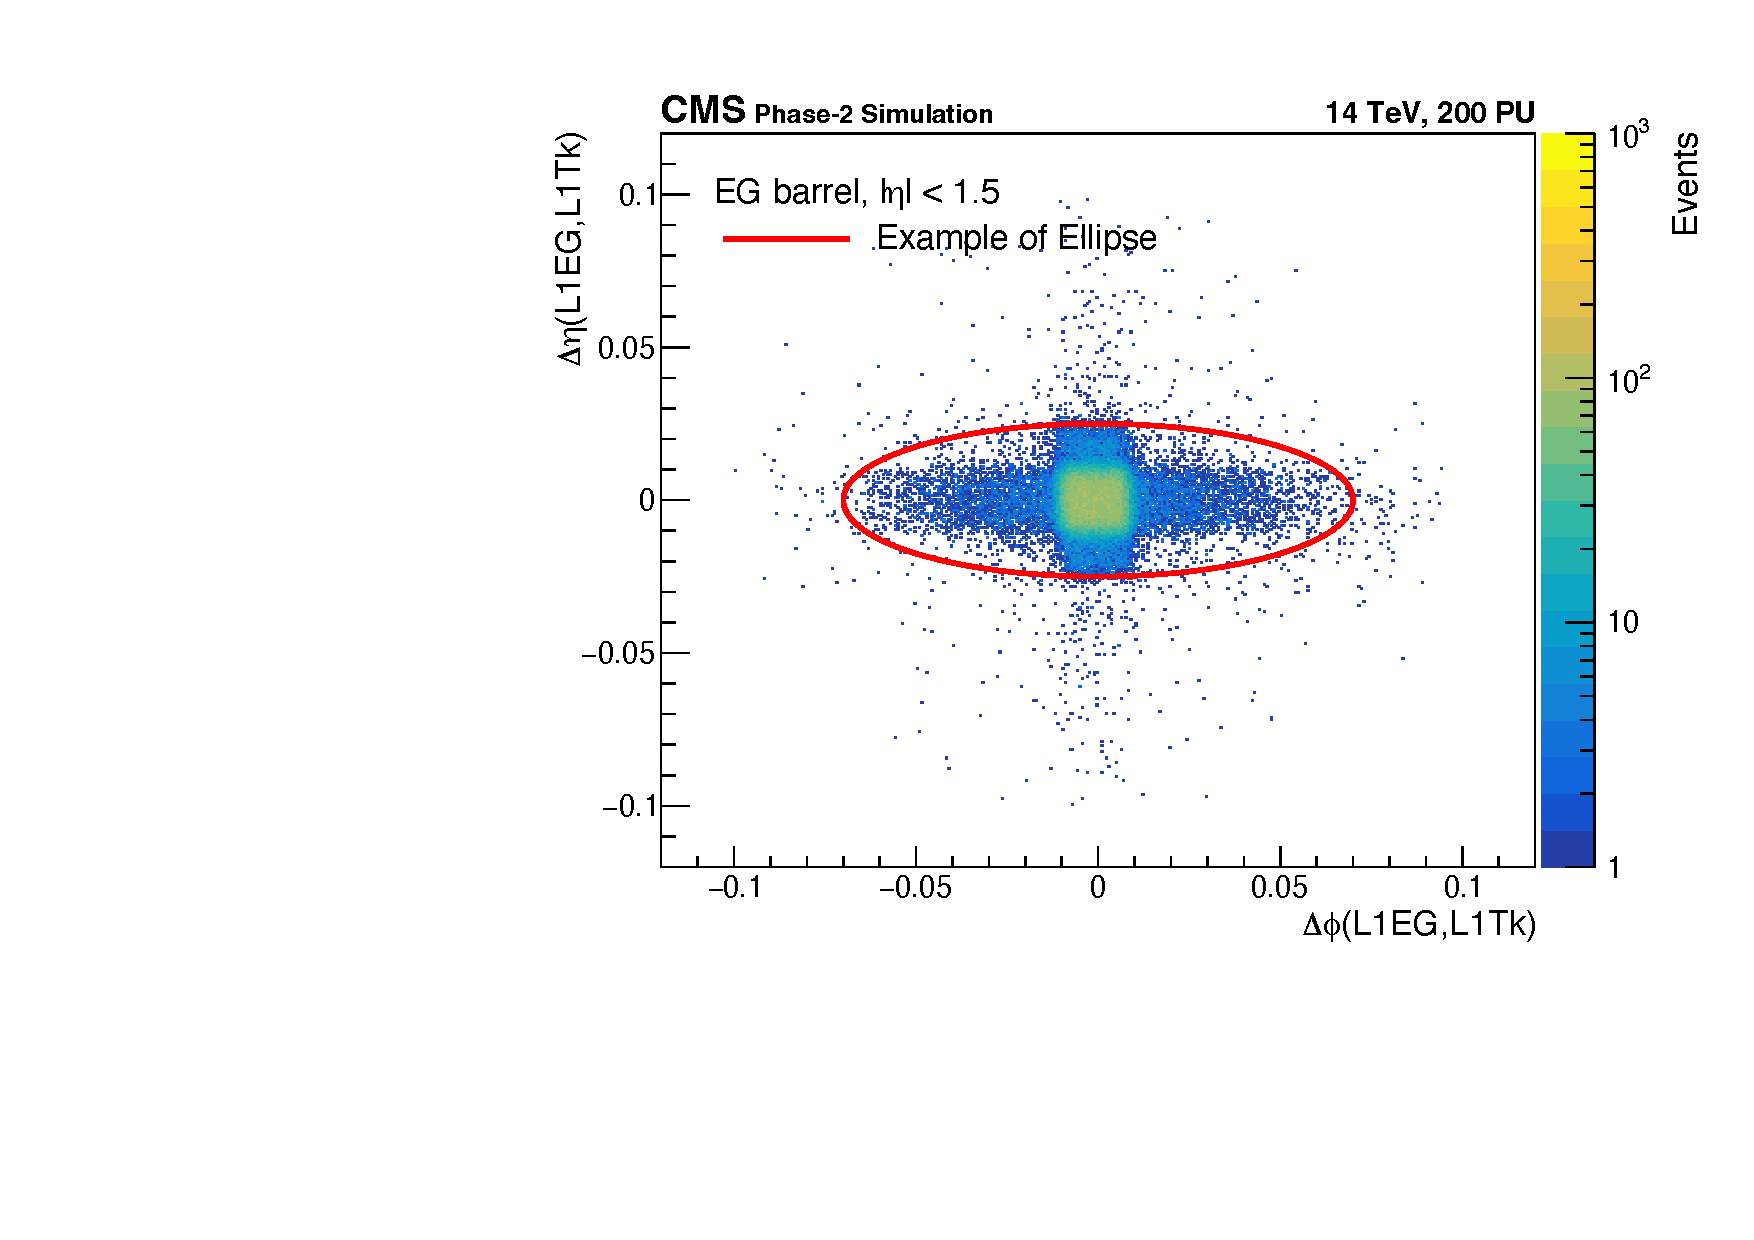
\includegraphics[width=.45\linewidth]{figures/Part2/Upgrade/DR_barrel}&
  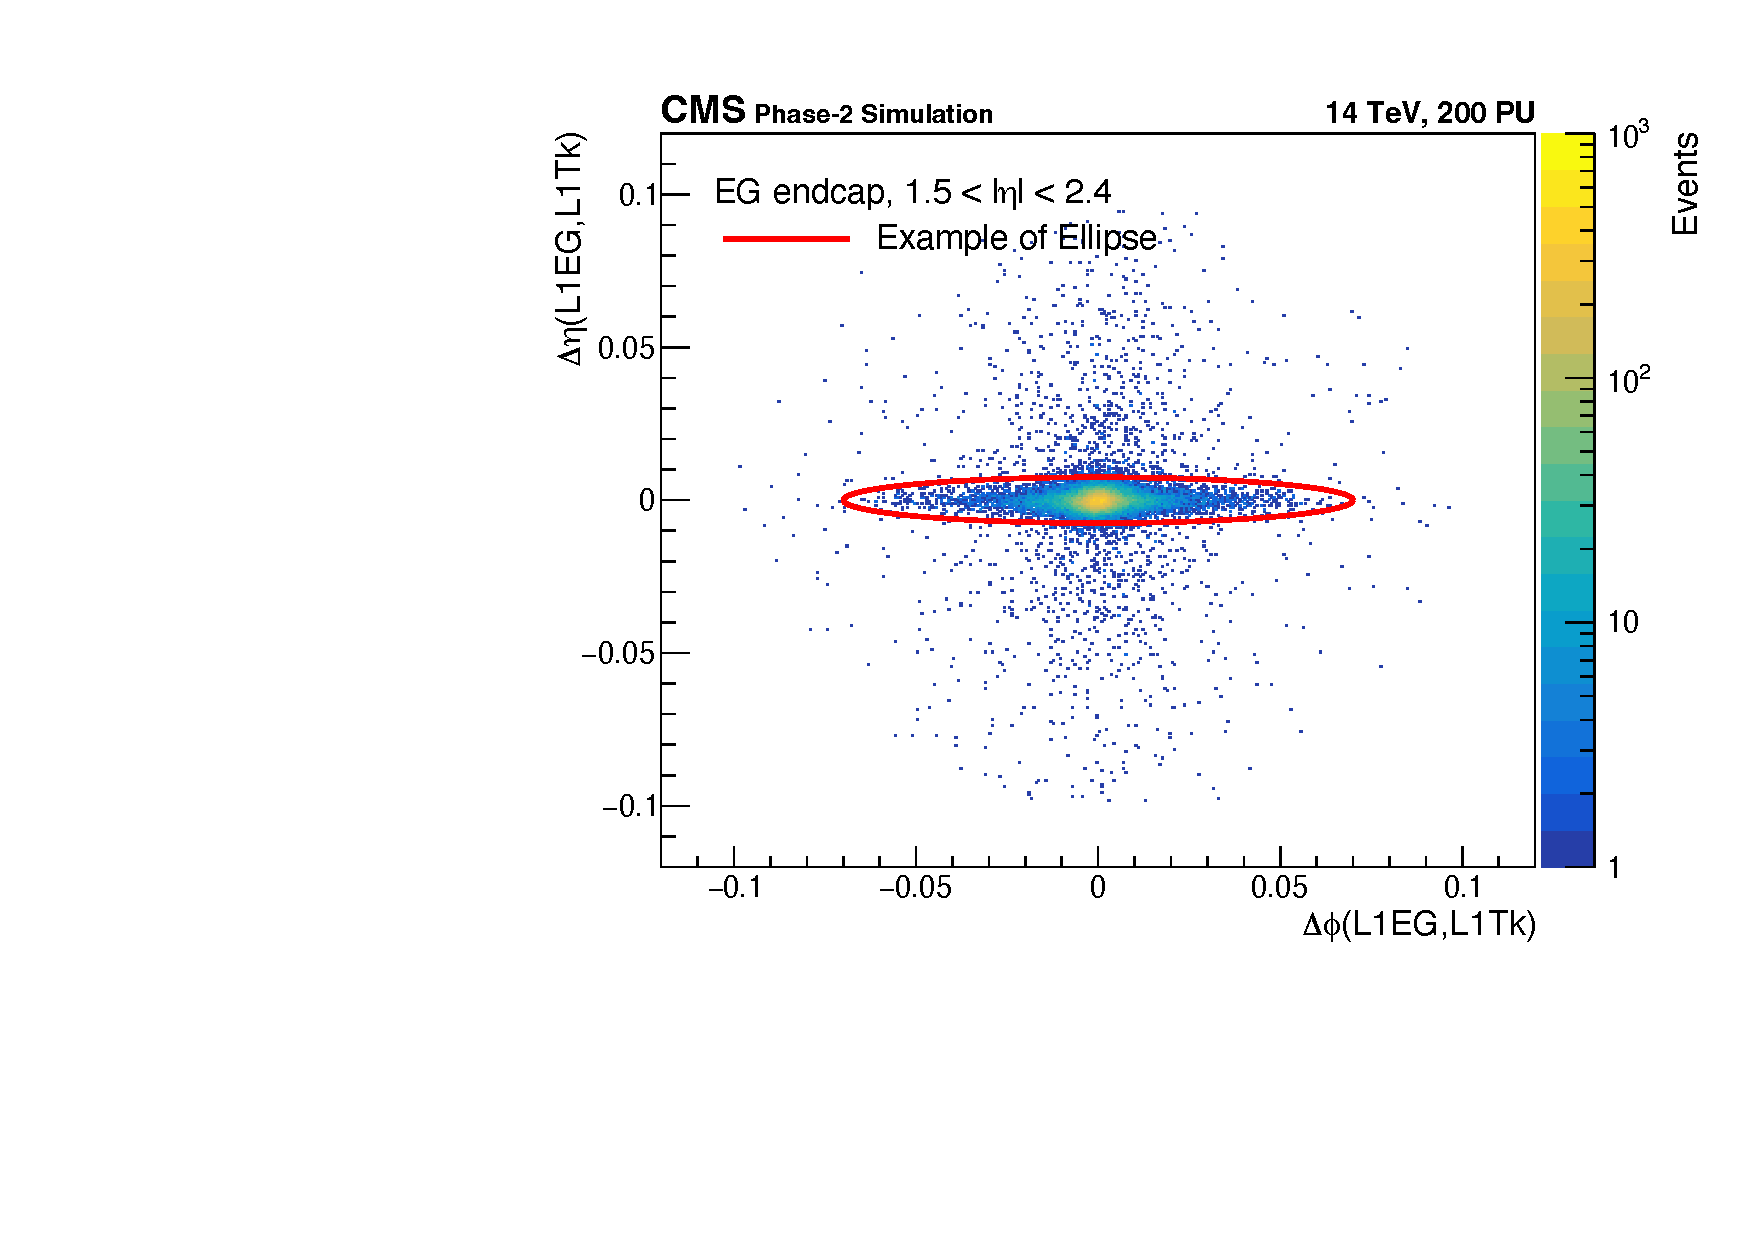
\includegraphics[width=.45\linewidth]{figures/Part2/Upgrade/DR_endcap}&
 \end{tabular}
 \caption{$\mathrm{\Delta}\eta$ vs $\mathrm{\Delta}\phi$ distances between calorimeter clusters and the closest \ac{L1} track in the \ac{ECAL} Barrel (left) and \ac{HGCAL}. Tracks are extrapolated using track $\pt$.}
 \label{fig:electron}
 \end{center}
\end{figure}

When compared to algorithms that only use calorimeter information, the baseline version of this new algorithm provides roughly a factor of three reduction in event rate while keeping the efficiency loss under control, as shown in Table~\ref{tab:L1EleRate}-Table~\ref{tab:L1EleEff}. The efficiency loss is largely driven by the inefficiencies in electron tracking, as illustrated in Figure~\ref{fig:electronperformance}.

\begin{table}[th]
\sffamily
\centering
\caption{Trigger rate of \ac{L1} trigger objects in the \ac{ECAL} Barrel. Data in the first column shows the two reference trigger thresholds.}
\begin{tabular}{ccc} \toprule
Rate & calorimeter only & track-matched \\  \midrule
 30 GeV   & 78.2 kHz   & 19.0 kHz\\ \midrule
 40 GeV & 25.5 kHz   & 8.3 kHz\\ \bottomrule
\end{tabular}
\label{tab:L1EleRate}
\end{table}

\begin{table}[th]
\sffamily
\centering
\caption{Trigger efficiency for \ac{L1} trigger objects computed at two reference trigger thresholds in the \ac{ECAL} Barrel. }
\begin{tabular}{ccc} \toprule
Efficiency & calorimeter only & track-matched \\  \midrule
 30 GeV   & 97.5\%   & 84.5\%\\ \midrule
 40 GeV & 98.7\%   & 88.0\%\\ \bottomrule
\end{tabular}
\label{tab:L1EleEff}
\end{table}

An alternative version of this algorithm uses the energy estimate from the calorimeter instead of the Outer Tracker to extrapolate \ac{L1} tracks. The superior energy resolution delivered by the calorimeters further constrains the projected track $\eta$ and $\phi$ coordinates to the targeted calorimeter clusters, as illustrated in \ref{fig:DR_electron}. This enables the implementation of a much tighter ellipse in the $\eta-\phi$ plane.

\begin{figure}[tbh!]
 \begin{center}
 \begin{tabular}{ccc}
  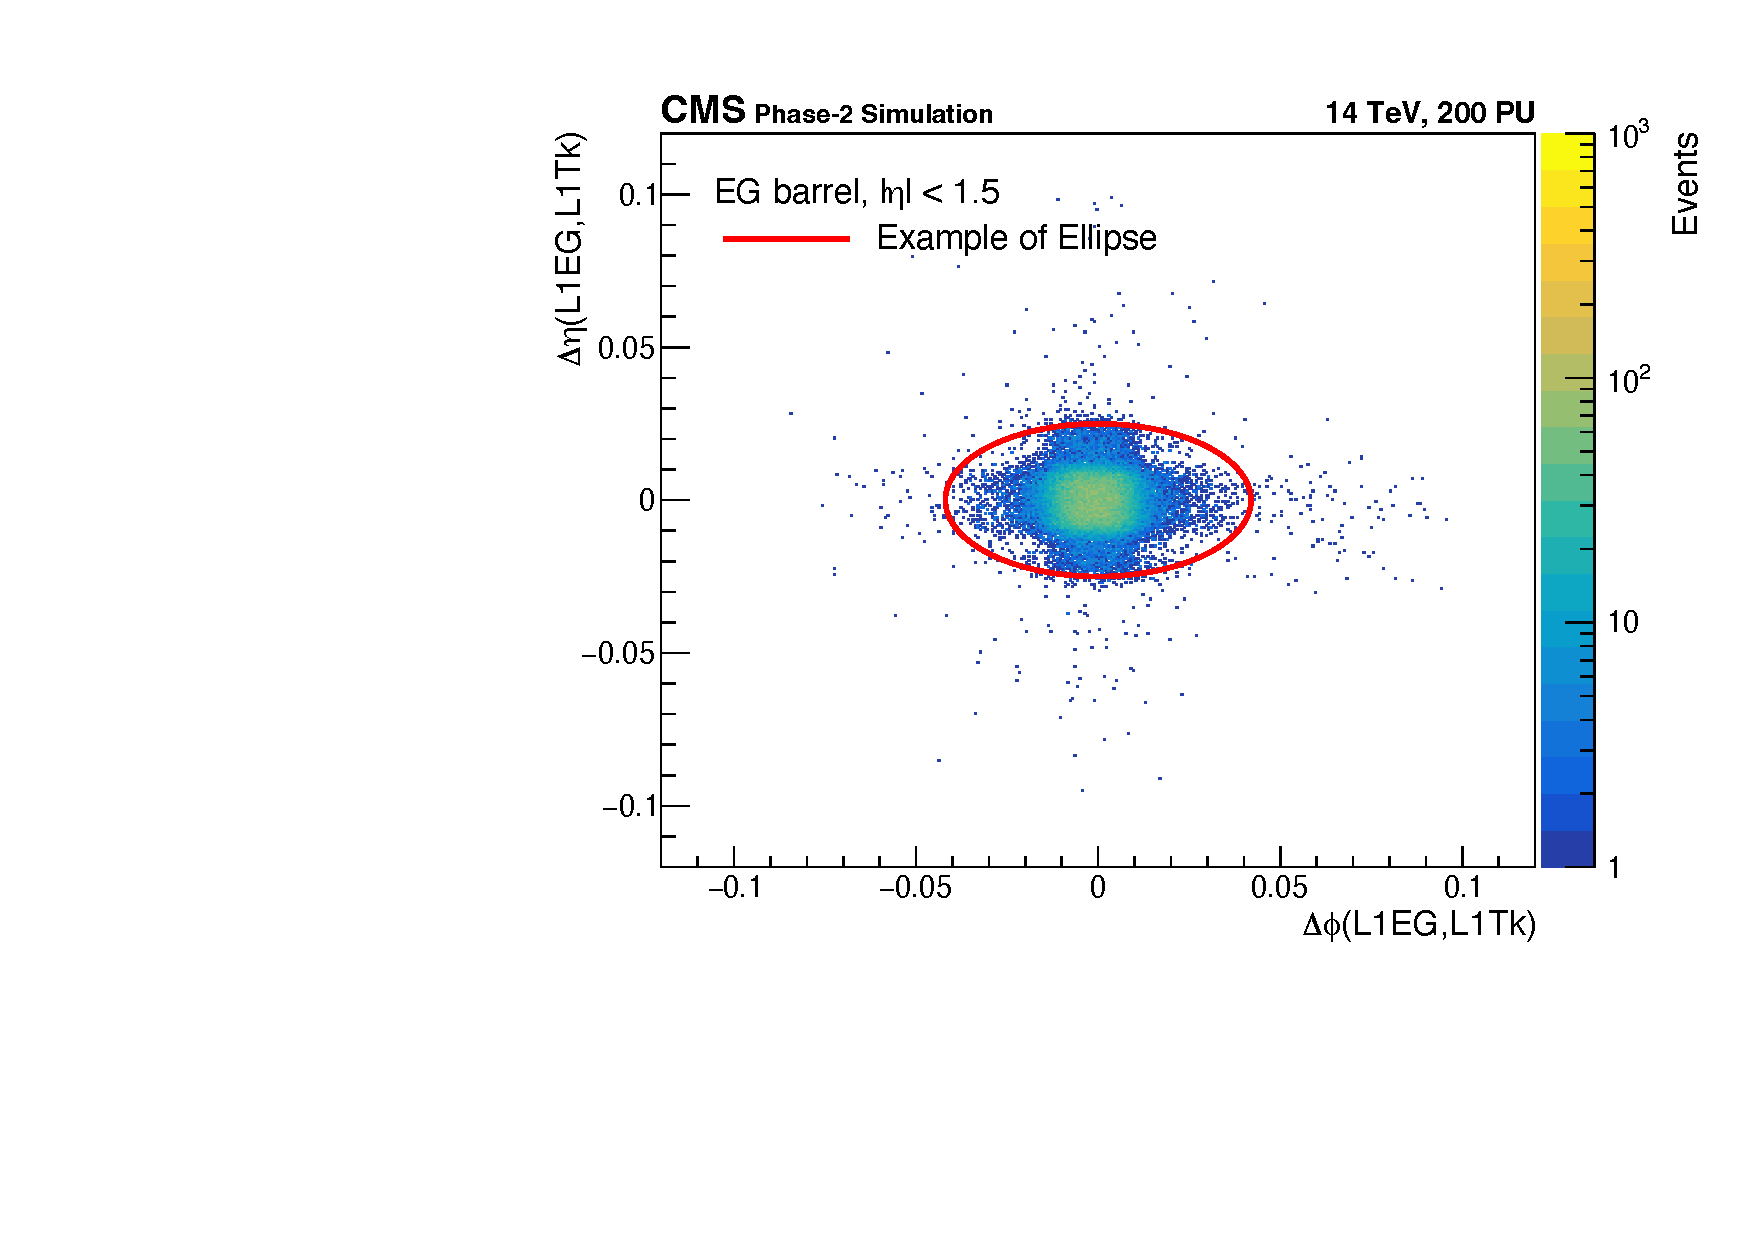
\includegraphics[width=.45\linewidth]{figures/Part2/Upgrade/DR_barrel_new}&
  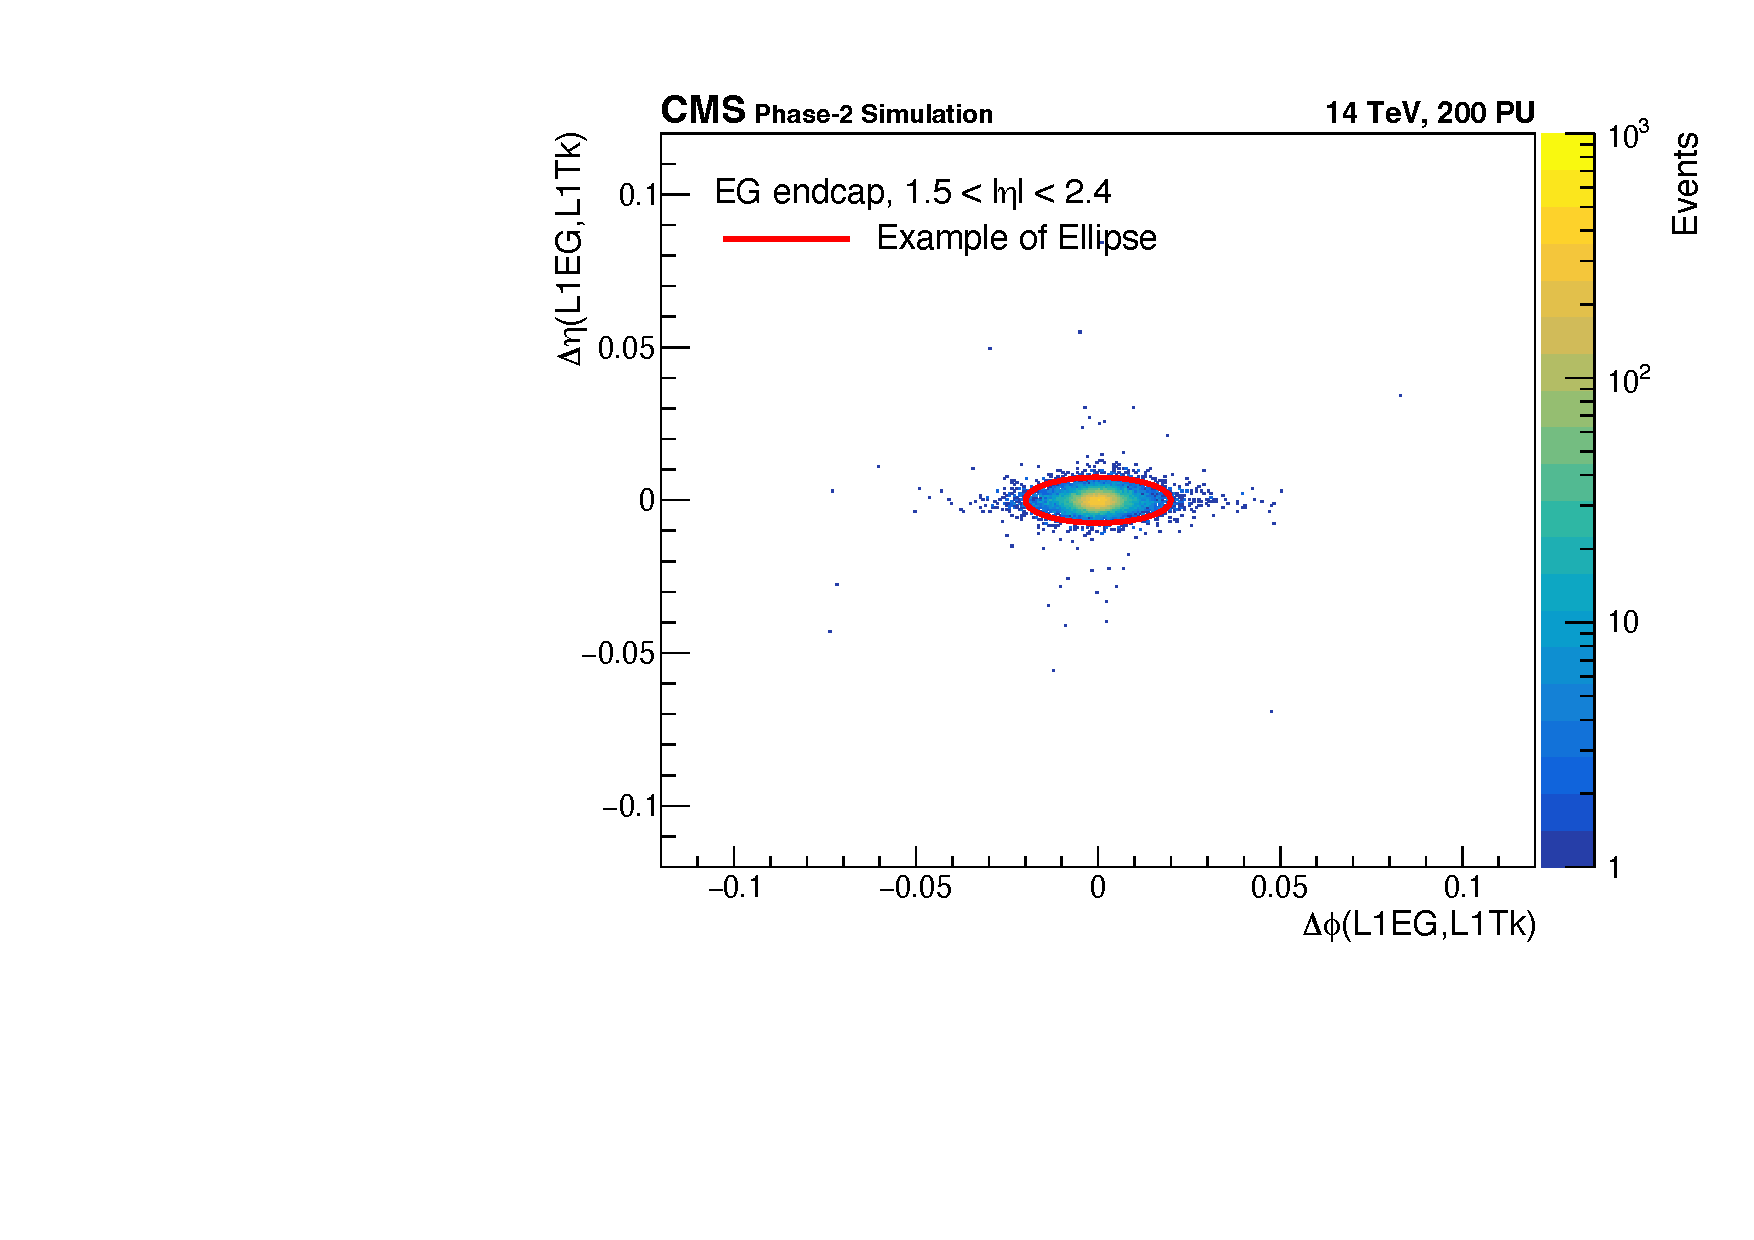
\includegraphics[width=.45\linewidth]{figures/Part2/Upgrade/DR_endcap_new}&
 \end{tabular}
 \caption{$\mathrm{\Delta}\eta$ vs $\mathrm{\Delta}\phi$ distances between calorimeter clusters and the closest \ac{L1} track in the \ac{ECAL} Barrel (left) and \ac{HGCAL}. Tracks are extrapolated using energy estimates from the calorimeter.}
 \label{fig:DR_electron}
 \end{center}
\end{figure}

A comparison between two versions of the electron trigger algorithms is shown in Figure~\ref{fig:rate_electron}-\ref{fig:eff_electron}. 

 \begin{figure}[tbh!]
 \begin{center}
 \begin{tabular}{ccc}
  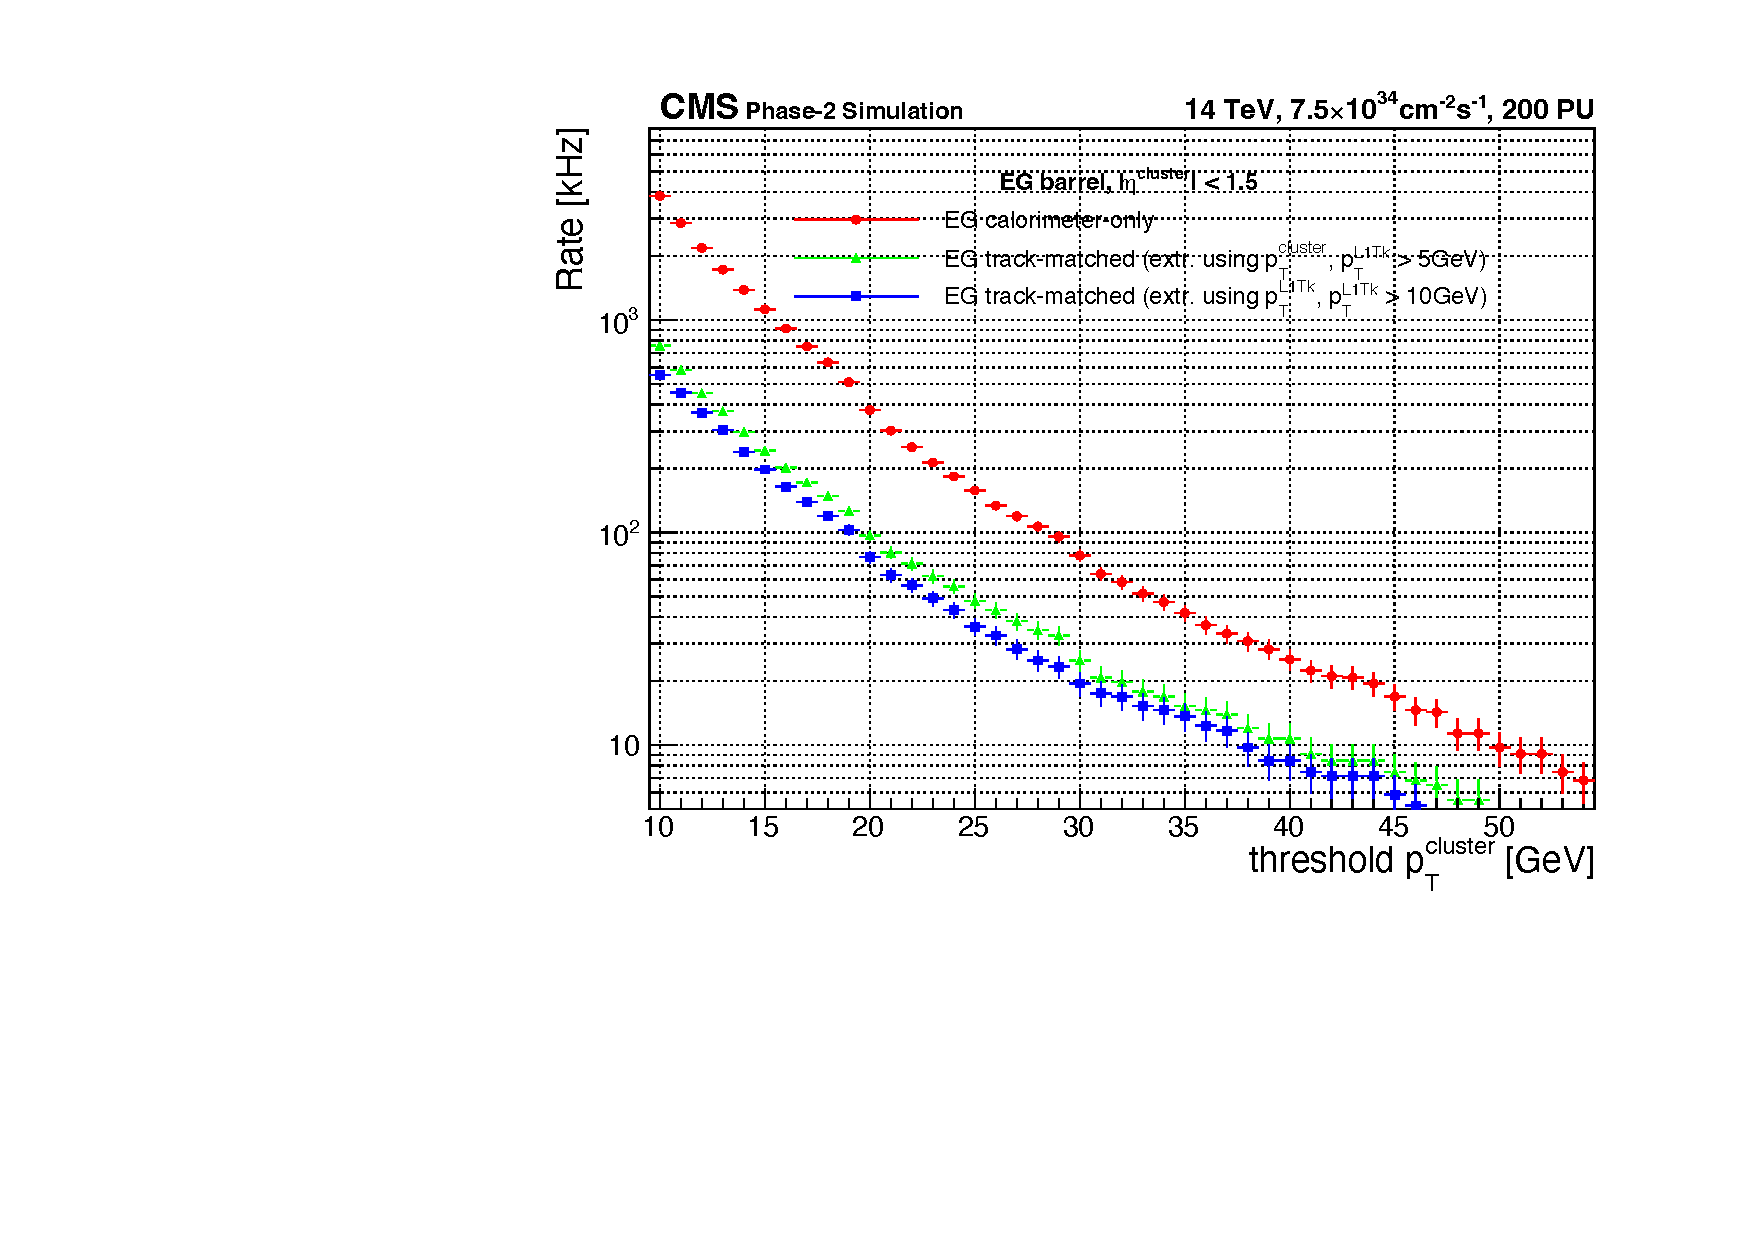
\includegraphics[width=.45\linewidth]{figures/Part2/Upgrade/Rate_barrel}&
  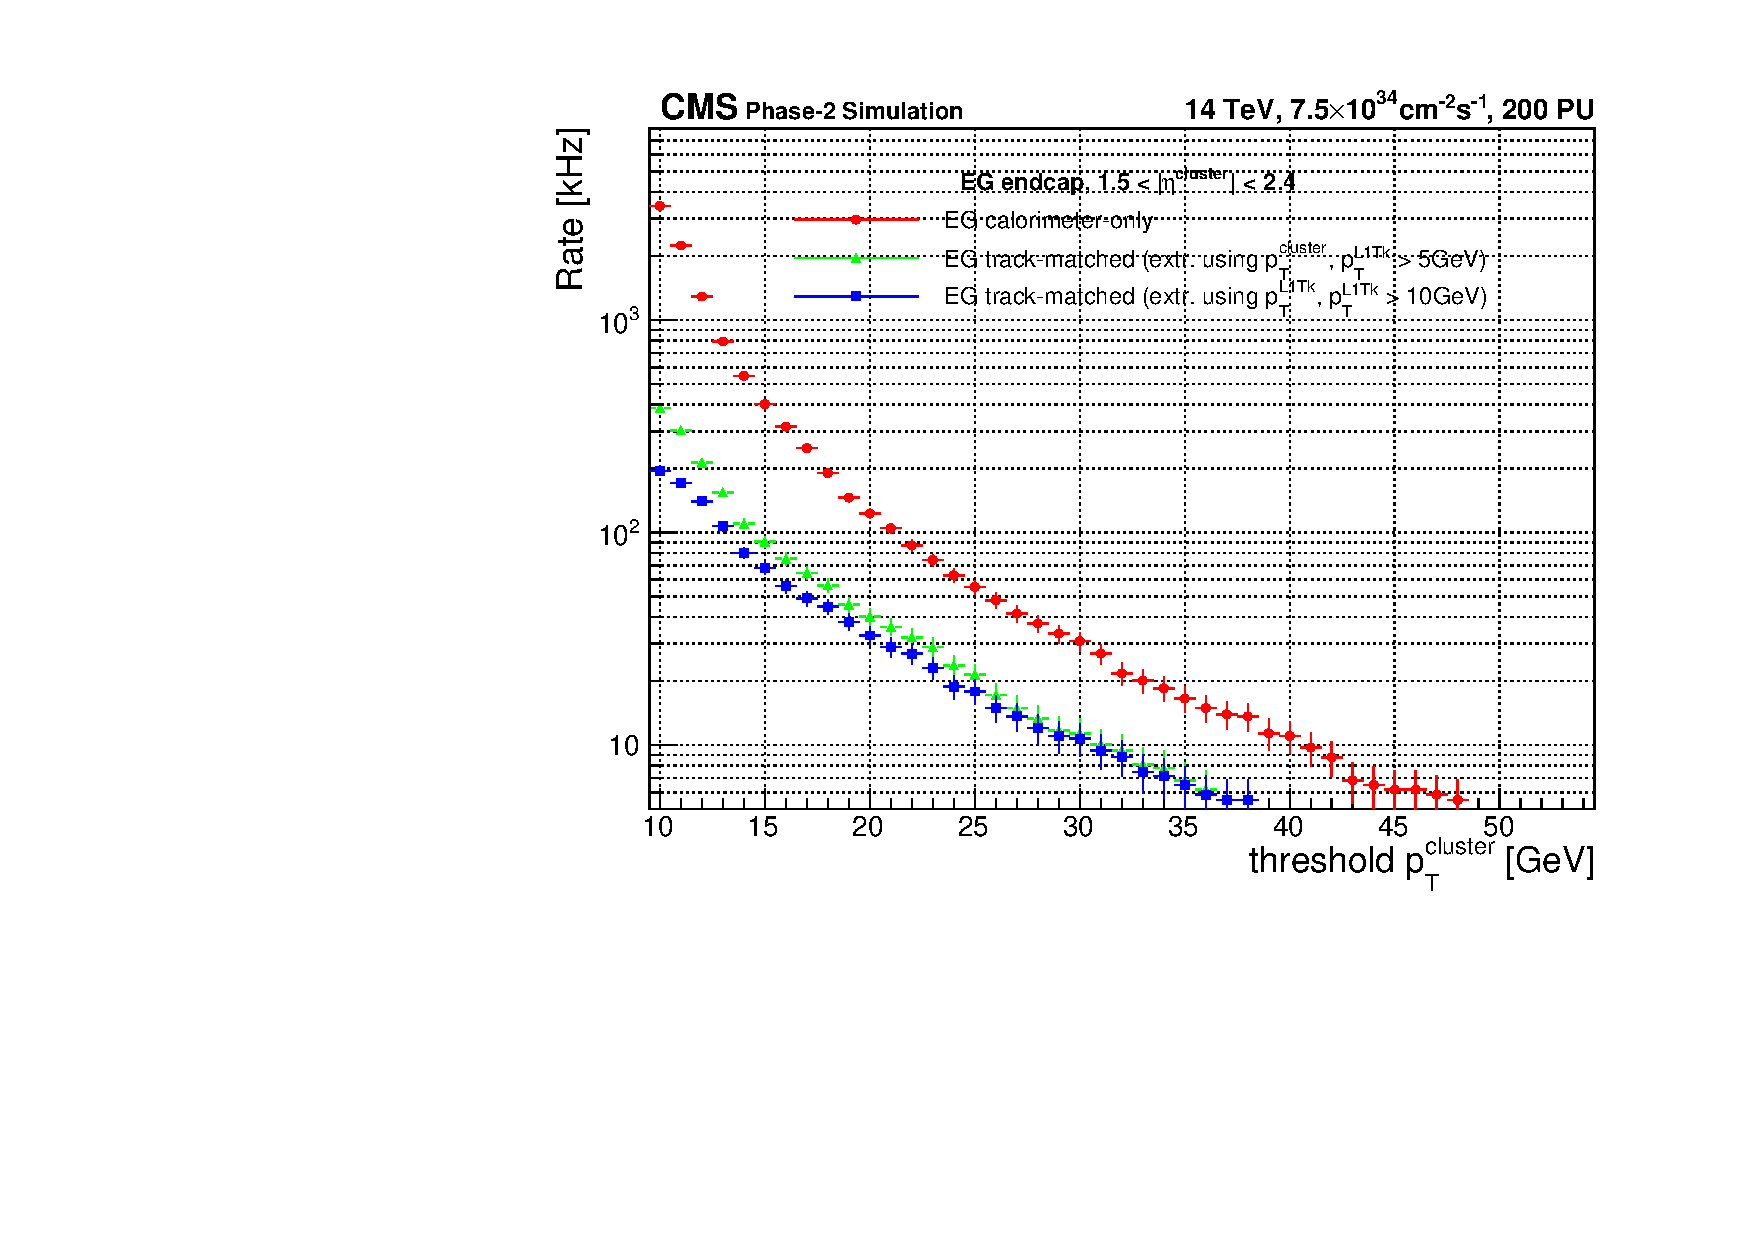
\includegraphics[width=.45\linewidth]{figures/Part2/Upgrade/Rate_endcap}&
 \end{tabular}
 \caption{\ac{L1} event rate as a function of the electron trigger threshold in the \ac{ECAL} Barrel (left) and \ac{HGCAL} (right). The event rate computed for calorimeter-only objects is shown in red data points. Event rates computed for the objects reconstructed by the baseline and alternative electron trigger algorithms are represented with blue and green data points, respectively.}
 \label{fig:rate_electron}
 \end{center}
\end{figure}

 \begin{figure}[tbh!]
 \begin{center}
 \begin{tabular}{ccc}
  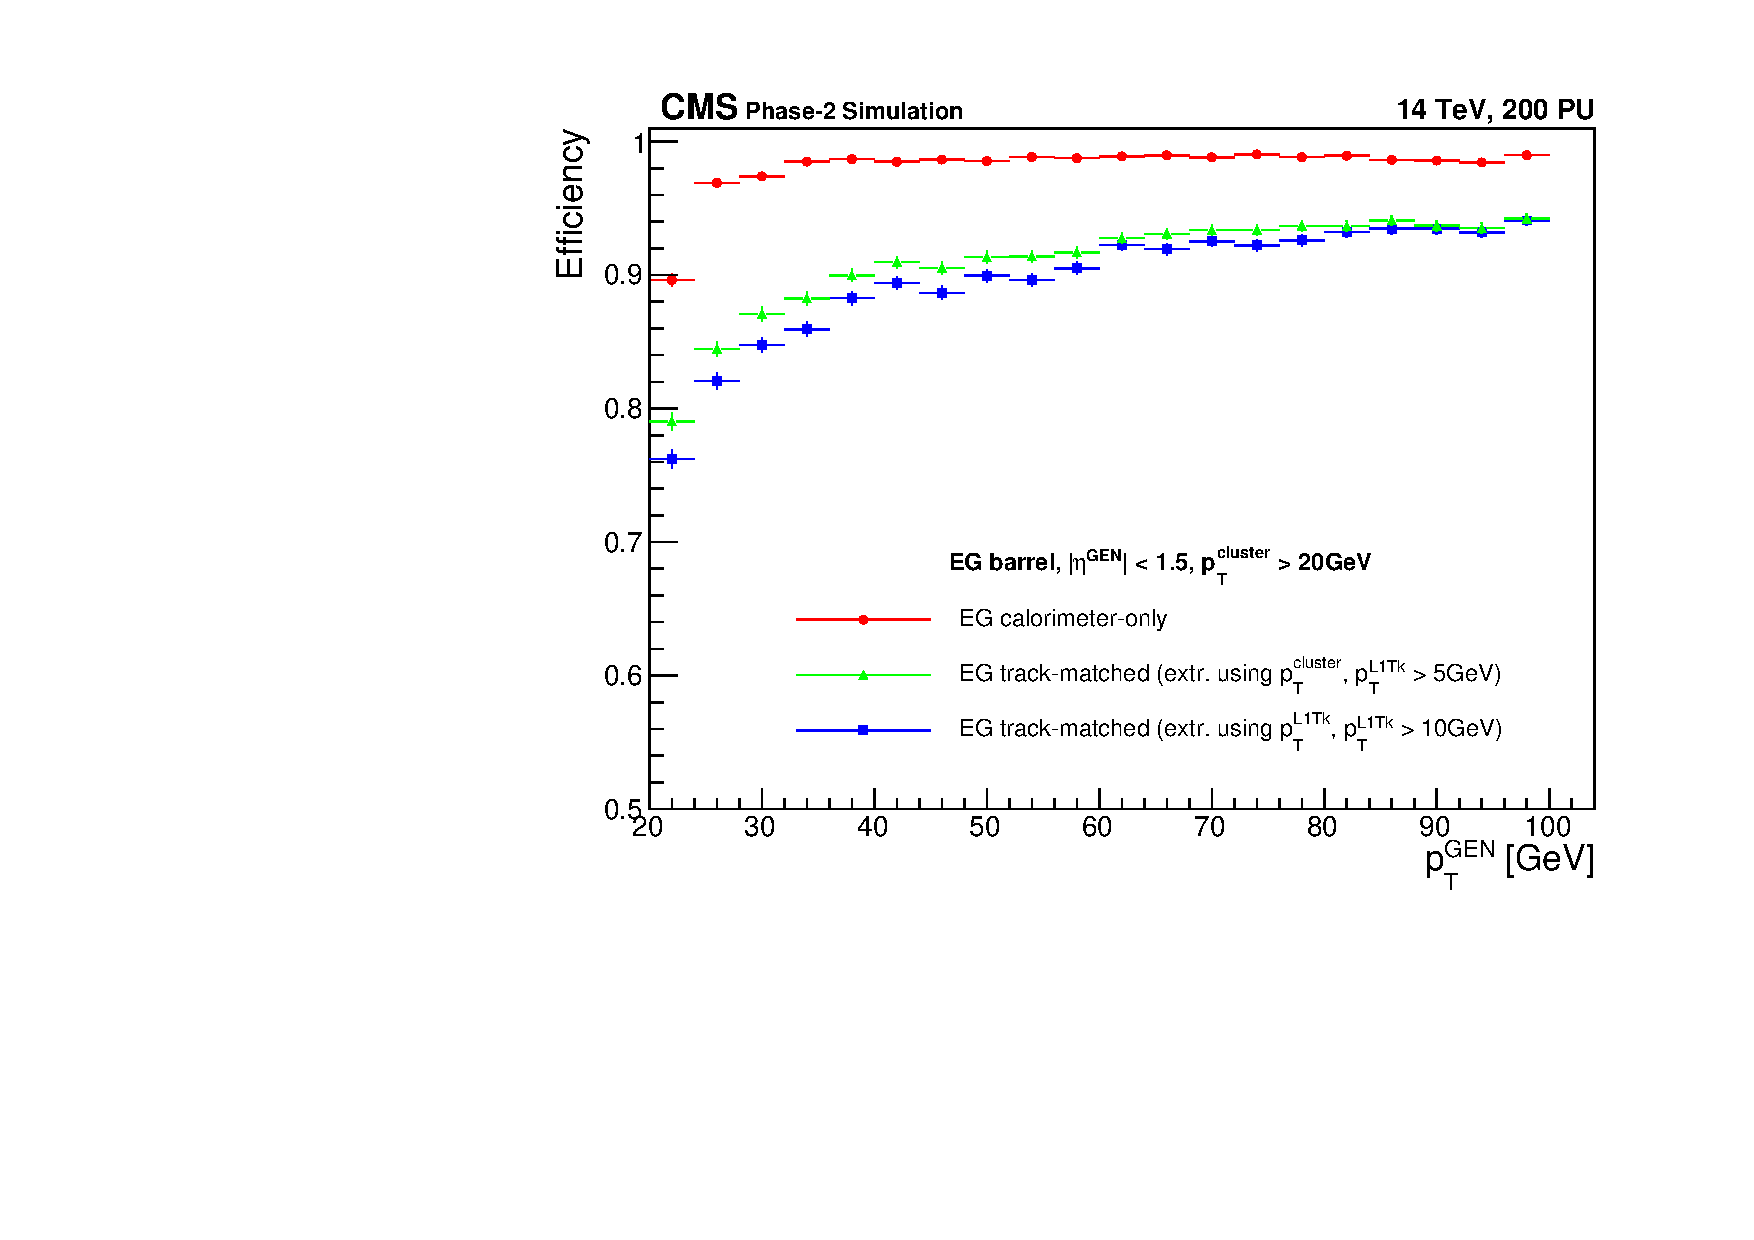
\includegraphics[width=.45\linewidth]{figures/Part2/Upgrade/eff_barrel}&
  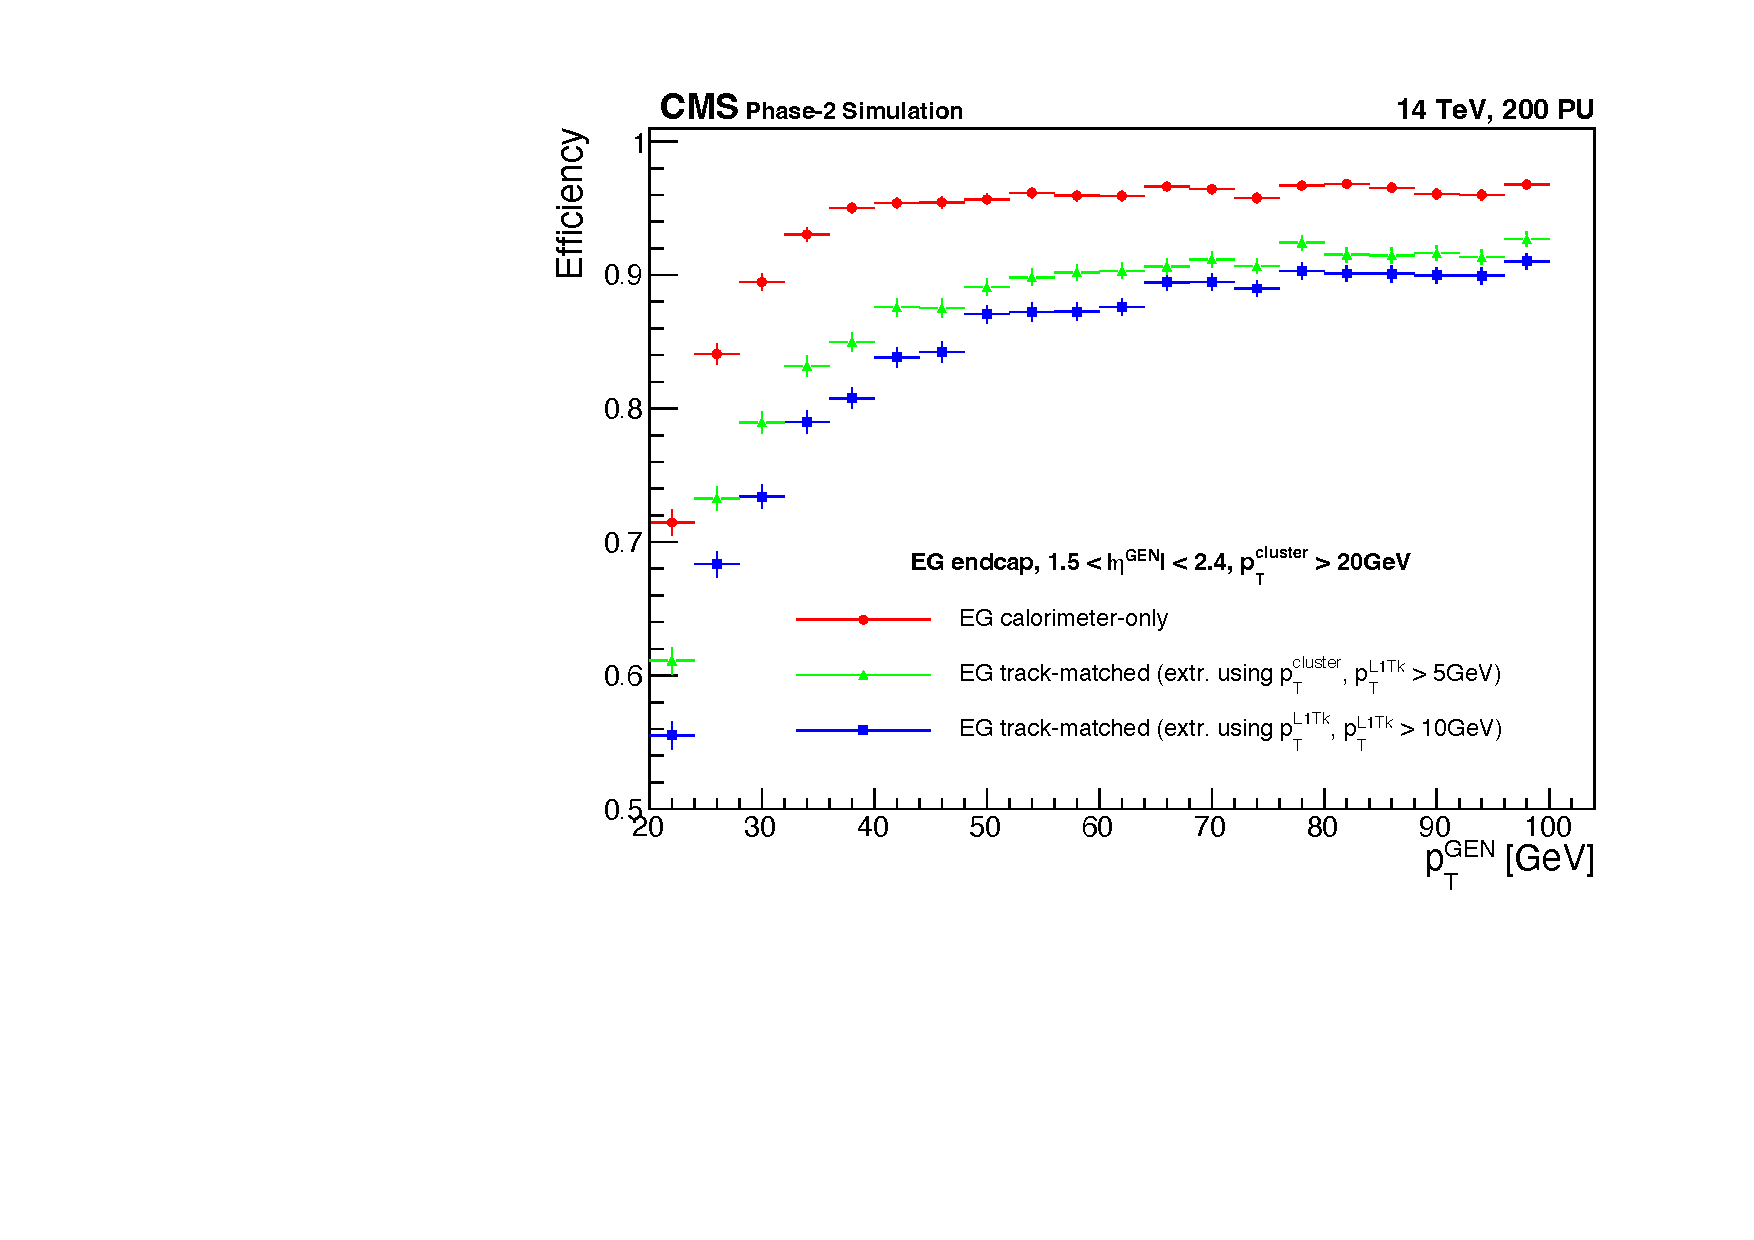
\includegraphics[width=.45\linewidth]{figures/Part2/Upgrade/eff_endcap}&
 \end{tabular}
 \caption{\ac{L1} electron trigger efficiency as a function of the particle $\pt$ in the \ac{ECAL} Barrel (left) and \ac{HGCAL} (right). The efficiency computed for calorimeter-only objects is shown in red data points. Efficiencies computed for the objects reconstructed by the baseline and alternative electron trigger algorithms are represented with blue and green data points, respectively.}
 \label{fig:eff_electron}
 \end{center}
\end{figure}

When compared to an older electron trigger algorithm for the Phase-2~\cite{Contardo:2015bmq}, this newly designed algorithm (baseline) improves the electron reconstruction efficiency at \ac{L1} by 5\% while reducing the background rate by a factor of 2. This improvement can be attributed to two main sources: (i) the improved matching scheme between tracks and calorimeter objects, and (ii) the improved performance in \ac{L1} track finder.